\documentclass[a4paper,parskip,11pt, DIV12]{scrreprt}

\usepackage[english]{babel} % FÌr Deutsch [english] zu [ngerman] Àndern. 
\usepackage[utf8]{inputenc}
\usepackage[T1]{fontenc}
\usepackage{blindtext}
\usepackage{graphicx}
\usepackage{subfigure}
%\renewcommand{\familydefault}{\sfdefault}
\usepackage{fancyhdr}
\usepackage{amsmath}
\usepackage{mdwlist} %Benötigt fÌr AbstÀnde in AufzÀhlungen zu löschen
\usepackage{here}
\usepackage{calc}
\usepackage{hhline}
\usepackage{marginnote}
\usepackage{chngcntr}
\usepackage{helvet}
\usepackage{tabularx}
\usepackage{titlesec} % TextÃŒberschriften anpassen
\setkomafont{sectioning}{\rmfamily}{\bfseries}

% \titleformat{Überschriftenklasse}[Absatzformatierung]{Textformatierung} {Nummerierung}{Abstand zwischen Nummerierung und Überschriftentext}{Code vor der Überschrift}[Code nach der Überschrift]

% \titlespacing{Überschriftenklasse}{Linker Einzug}{Platz oberhalb}{Platz unterhalb}[rechter Einzug]

\titleformat{\chapter}{\LARGE\bfseries}{\thechapter\quad}{0pt}{}
\titleformat{\section}{\Large\bfseries}{\thesection\quad}{0pt}{}
\titleformat{\subsection}{\large\bfseries}{\thesubsection\quad}{0pt}{}
\titleformat{\subsubsection}{\normalsize\bfseries}{\thesubsubsection\quad}{0pt}{}

\titlespacing{\chapter}{0pt}{-2em}{6pt}
\titlespacing{\section}{0pt}{6pt}{-0.2em}
\titlespacing{\subsection}{0pt}{5pt}{-0.4em}
\titlespacing{\subsubsection}{0pt}{-0.3em}{-1em}

%\usepackage[singlespacing]{setspace}
%\usepackage[onehalfspacing]{setspace}

\usepackage[
			%includemp,				%marginalien in Textkörper einbeziehen
			%includeall,
			%showframe,				%zeigt rahmen zum debuggen		
			marginparwidth=25mm, 	%breite der marginalien
			marginparsep=5mm,		%abstand marginalien - text
			reversemarginpar,		%marginalien links statt rechts
			%left=50mm,				%abstand von Seitenraendern
%			top=25mm,				%
%			bottom=50mm,
			]{geometry}		

%Bibliographie- Einstellungen
\usepackage[babel,german=quotes]{csquotes}
\usepackage[
   backend=bibtex8, 
   natbib=true,
    style=numeric,
    sorting=none
]{biblatex}
\bibliography{Quelle}
%Fertig Bibliographie- Einstellungen

\usepackage{hyperref}

\newcommand{\footnoteremember}[2]{
  \footnote{#2}
  \newcounter{#1}
  \setcounter{#1}{\value{footnote}}
}
\newcommand{\footnoterecall}[1]{%
  \footnotemark[\value{#1}]
}

\MakeRobust{\ref}% avoid expanding it when in a textual label

\makeatletter
\newcommand{\labeltext}[2]{%
  \@bsphack
  \csname phantomsection\endcsname % in case hyperref is used
  \def\@currentlabel{#1}{\label{#2}}%
  \@esphack
}
\makeatother
	
\begin{document}
	
	\begin{titlepage}
		\begin{figure}[H]
			\hfill
			\subfigure{
\includegraphics[scale=0.04]{uzh}}
		\end{figure}
		\vspace{1 cm}
		\textbf{\begin{huge}KT I Lab Course
		\end{huge}}\\
		\noindent\rule{\textwidth}{1.1 pt} \\
		
		\begin{Large}\textbf{Angular Correlation}
		\end{Large}\\ 
		\normalsize 
		\par
		\begingroup
		\leftskip 0 cm
		\rightskip\leftskip
		\textbf{Assistant:}\\ Alexander Kish \\ \\
		\textbf{Students:}\\ Fabian Stäger, Manuel Sommerhalder \\ \\
		\textbf{Date of experiment:}\\ 24.01.2018 \\ \\
		\par
		\endgroup
		\clearpage
		
		
		
	\end{titlepage}
	
%Start Layout
	\pagestyle{fancy}
	\fancyhead{} 
	\fancyhead[R]{\small \leftmark}
	\fancyhead[C]{\textbf{Angular Correlation} } 
	\fancyhead[L]{
\includegraphics[height=2\baselineskip]{uzh}}
	
	\fancyfoot{}
	\fancyfoot[R]{\small \thepage}
	\fancyfoot[L]{}
	\fancyfoot[C]{}
	\renewcommand{\footrulewidth}{0.4pt} 
	
	\addtolength{\headheight}{2\baselineskip}
	\addtolength{\headheight}{0.6pt}
	
	
	\renewcommand{\headrulewidth}{0.6pt}
	\renewcommand{\footrulewidth}{0.4pt}
	\fancypagestyle{plain}{				% plain redefinieren, damit wirklich alle seiten im gleichen stil sind (ausser titlepage)
		\pagestyle{fancy}}
	
	\renewcommand{\chaptermark}[1]{ \markboth{#1}{} } %Das aktuelle Kapitel soll nicht Gross geschriben und Nummeriertwerden
	
	\counterwithout{figure}{chapter}
	\counterwithout{table}{chapter}
	%Ende Layout
	
	\tableofcontents
	
\chapter{Introduction}

		The goal of this experiment is to measure the angular correlation function of $\gamma$-rays in a $^{60}$Co decay and compare it to theoretical predictions.

\section{The $^{60}$Co Decay}

		$^{60}$Co is a synthetic isotope of cobalt with a half-life of 5.1 years. Through $\beta ^-$ decay it disintegrates into an excited $^{60}$Ni atom with an energy of 2505 keV and $l$ = 4 with positive parity. This nickel isotope thus emits two successive gamma rays with energies of 1172 keV and 1332 keV in order to reach its stable state of 0$^{+}$. Since the intermediate state (2$^+$) has a lifetime of around 1 ps, the two $\gamma$-rays can due to the finite experimental time resolution be treated as coincident. A schematic diagram of the $^{60}$Co decay is provided in figure \ref{fig:CoDecay}.	
\begin{figure}[H]
\centering
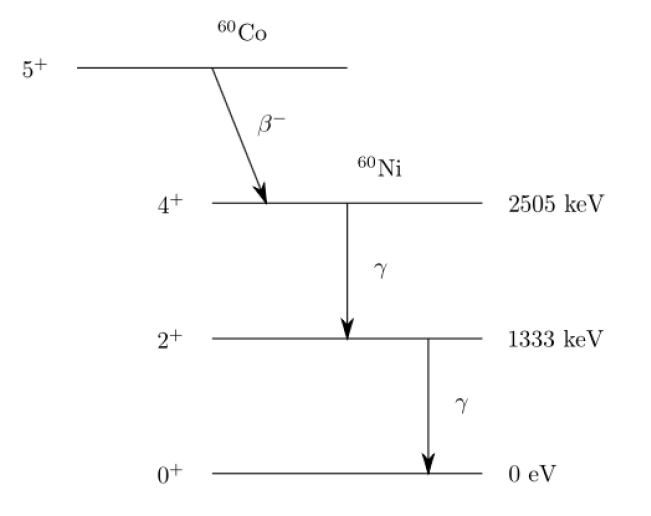
\includegraphics[scale=0.65]{60CoDecay.png}
\caption[60CoDecay]{Schematic illustration of the $^{60}$Co Decay. [\ref{source:manual}]}
\label{fig:CoDecay}
\end{figure}
		
\section{Angular Correlation}

		The two successive $\gamma$-rays are predicted to be emitted anisotropically relative to each other according to the general angular correlation function [\ref{source:manual}]:
		\begin{equation}
		W(\theta) = 1 + \sum^l_1 a_i \cos ^{2i} \theta
		\end{equation}	
		This function describes the probability for the latter gamma ray to be emitted at an angle $\theta$ from the first one. 2$l$ is the order of the lowest multipole in the cascade. In case of the $^{60}$Co decay, both gamma rays are emitted during a transision of $\Delta l$ = 2 and positive parity, so the dominant contribution is the electric quadrupole and the correlation function reduces to:	
		\begin{equation} \label{eq:Ang1}
		W(\theta) = 1 + a_1 \cos ^{2} \theta +  a_2 \cos ^{4} \theta
		\end{equation}		
		The coefficients $a_1$ and $a_2$ have been theoretically predicted by Dr. Hamilton [\ref{source:Hamilton}] for all combinations of angular momenta involved by consideration of state transitions using the Clebsch-Gordan-coefficients. These are summarized in figure \ref{fig:coefficients}		
		\begin{figure}[H]
\centering
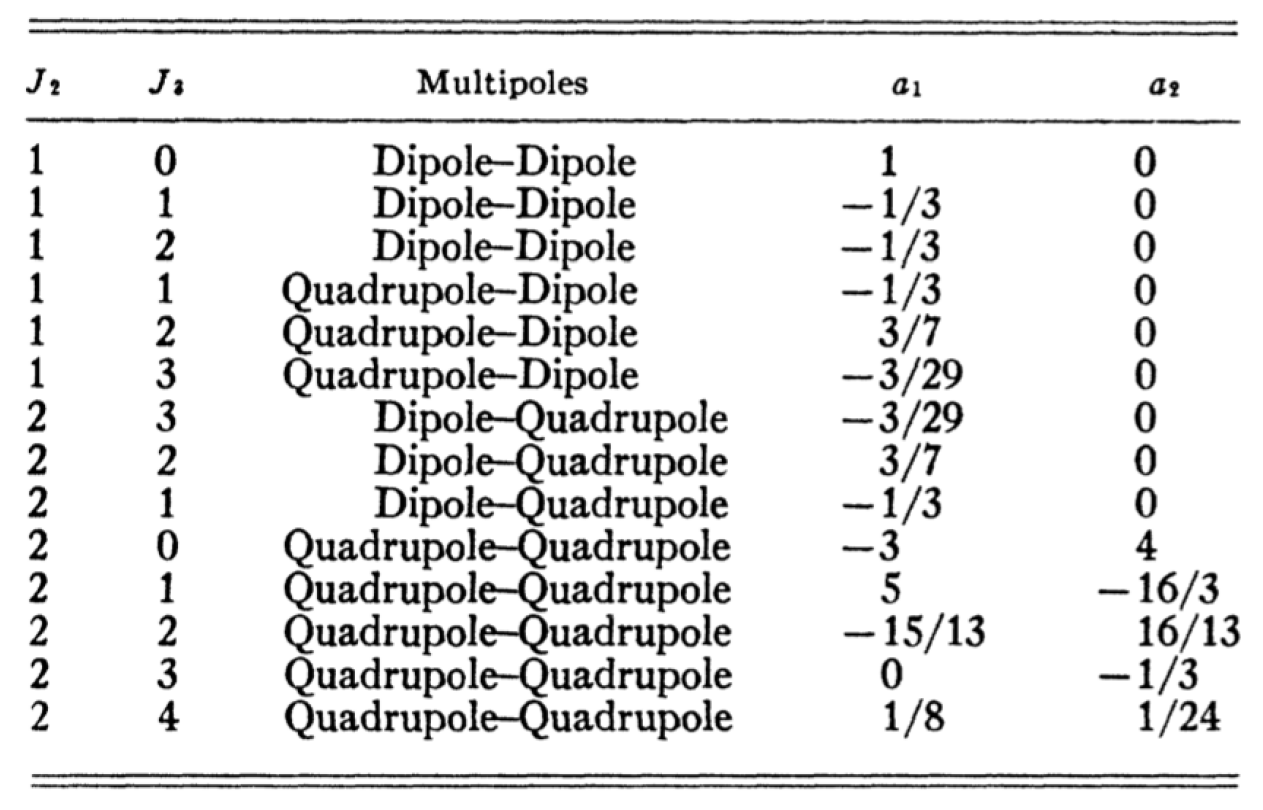
\includegraphics[scale=0.4]{Coefficients.png}
\caption[Coefficients]{Coefficients $a_1$ and $a_2$ for different combinations of $J_1$ and $J_2$ for an atom deexciting into the ground state $J_1$ = 0 [\ref{source:manual}]}
\label{fig:coefficients}
		\end{figure}		
		Since the angular momenta of $J_3$ = 4, $J_2$ = 2, $J_1$ = 0 are assumed for the $^{60}$Co decay, the expected correlation function has the following explicit form:		
		\begin{equation} \label{eq:AngularCorrelation}
		W(\theta) = 1 + \frac{1}{8} \cos ^{2} \theta +  \frac{1}{24} \cos ^{4} \theta
		\end{equation} 
		
\section{Experimental Concept}

		The experimental setup, more throroughly described in section \ref{sec:setup}, consists of two scintillation counters that detect the coincident $\gamma$-rays from different and adjustable relative angles. The rate of detected events is then plotted and compared to the theoretical description from formula \ref{eq:AngularCorrelation}.
		
\chapter{Measurement Principle}	

\section{Experimental Set-Up} \label{sec:setup}

		The $^{60}$Co-sample is placed in the center of a goniometer table where a large scintillation counter $D_l$ is set up at a fixed position, measured to be at a distance of $r_l$ = 216 mm from the sample, pointing to the center. A smaller scintillation counter $D_s$ is mounted on a rotatable arm, also pointing to the center. The angle relative to the fixed detector can be read off the edge of the goniometer table. The distance $r_S$ from the small detector to the sample can be adjusted. Here we chose 87 mm in order to achieve the same solid angle coverage as the large detector. This was deduced from the definition of the solid angle:\begin{eqnarray}
&\Omega  = \frac{A}{r^2} = \frac{\pi}{4} \frac{d^2}{r^2} \\
&\Omega_l = \Omega_s \quad \iff \quad r_s = \frac{d_s}{d_l} r_l
\end{eqnarray} with diameters $d_l$ = 139 mm for the large detector and $d_s$ = 56 mm for the small one. The high-voltage bias for the two detectors were set to $U_l$ = 1400 V for $D_l$ and $U_s$ =1000 V for $D_s$. The gains of the amplifiers to 35 for $D_l$ and 69 for $D_s$. 

The signal from each detector is split into two branches which will be called the 'energy branch' and the 'time branch' (see figure \ref{fig:Electronics1}). The modules in these branches are briefly characterized in section \ref{sec:modules}. The idea behind the 'time branch' is to record any coincident signal with the corresponding deviation from exact coincidence, which is expected to be gaussian distributed. Since the expectation value of the time delay between coincident events is zero and the time-to-amplitude converter (TAC) cannot record negative delays, the $D_s$-signal is shifted by a time that is large compared to the expected deviations.  The 'energy branch' is supposed to eliminate random coincidents by opening the gate of the multichannel analyzer (MCA) for the 'time branch' signals only when the same event is measured by both detectors.
\begin{figure}[H]
\centering
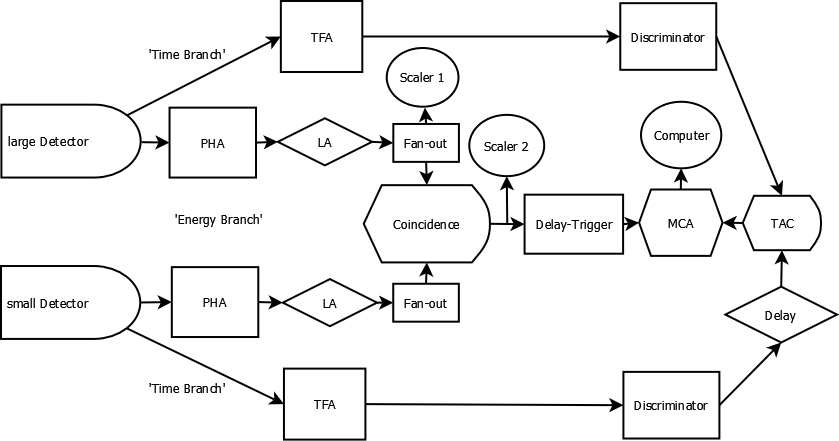
\includegraphics[width=1\textwidth]{KT-Elektronik.png}
\caption[Electronics1]{Flowchart showing all the electronic modules used for processing the detector signals}
\label{fig:Electronics1}
		\end{figure}
The 'time branch' starts at each detector with a timing filter amplifier (TFA) which is used to turn the detector signal into a clear analog signal. This signal is subsequently turned into a digital NIM pulse in a discriminator. The signal originating from $D_l$ is forwarded into the start-channel of a TAC. The signal from $D_s$, on the other hand, is first delayed in a delay module by $t_0$ = 48 ns before being forwarded into the stop-channel of the TAC, which transfers a pulse to the ADC-channel of the MCA with an amplitude proportional to the time delay between the two incoming signals. 

 The 'energy branch' starts at each detector with an amplifier containing a pulse height analyzer (PHA). The signal produced by the detectors represents a broad energy spectrum (see section \ref{sec:EnergySpectrum}). Since only the $\gamma$-decays are of interest, the window of the PHA is set such that only the TTL pulses corresponding to the $\gamma$-ray emission are passed to the level adapter (LA), where they are converted into NIM signals. After the conversion, they pass a fan-out module where the signal of the $D_l$ is split into two identical pulses and one of them enters a scaler S1 that counts the rate of events. This data is used for a cross-check of the measurement. The signals of the two detectors merge into an AND-gate inside a coincidence module. This module returns a pulse only if there is a signal coming from both detectors at the same time. The output signal is then forwarded into another scaler S2, which is also used for cross-checking, and into a delay-trigger that generates a rectangular TTL signal with adjustable delay and width. This signal is used as the gate input for the MCA.

The computer connected to the MCA records the number of events contained in a histogram where the bins correspond to the delay between the detector signals. This measurement is performed while placing the small detector at different angles $\theta$ relative to the large one, covering a $\theta$-range from 180$^\circ$ to 60$^\circ$ with decrements of 15$^\circ$. Each measurement will last for 20 min. In order to be able to assign an actual time delay to each bin in the histogram, a calibration measurement is carried out where the output of the TAC is observed for different known delays (see section \ref{sec:TimeCal}). 


\section{Electronic Modules} \label{sec:modules}

A short description [\ref{source:manual}] for each electronic moudule used during the experiment is listed here, followed by two photographs showing the actual set-up, previously only illustrated schematically in figure \ref{fig:Electronics1}.

The \textbf{pulse height analyser} (PHA) module creates a TTL output signal for every input signal inside a predifined range.
\\
The \textbf{timing filter amplifier} (TFA) allows to adjust the shape of a signal according to  the desired tinme constants.
\\
The \textbf{discriminator} turns an analog input signal above a certain threshold into a logic (NIM) pulse whose width is adjustable.
\\
The \textbf{level adapter} (LA) converts logic TTL signals into NIM signals or the other way around.
\\
The \textbf{fan-out} module splits an input signal into several identical output signals.
\\
The \textbf{coincidence module} contains a logic AND-gate that generates a NIM pulse whenever there is a signal on all input channels.
\\
The \textbf{scaler} counts the number of incoming signals. 
\\
The \textbf{delay module} is a passive module that delays the incoming signal by a desired amount of time.
\\
The \textbf{delay trigger} turns a rectangular input signal into an output signal with adjustable length and delay.
\\
The \textbf{time-to-amplitude-converter} (TAC) returns a pulse whose amplitude is proportional to the time delay between the signal at the start channel and the signal at the stop channel
\\
The \textbf{multichannel analyser} (MCA) takes pulses of different amplitudes as input and returns a histogram that counts the number of pulses per amplitude. It also contains a Gate channel which allows to register an event signal only when there is a signal on the Gate channel.
\\
In this experiment, two different kinds of logic pulses are used. A TTL signal has a baseline of +/- 0.5V and is a rectangular pulse corresponds to a voltage of 5V. A NIM signal, on the other hand, is interpreted as a pulse when it falls to -800mV.

\begin{figure}[H]
\centering
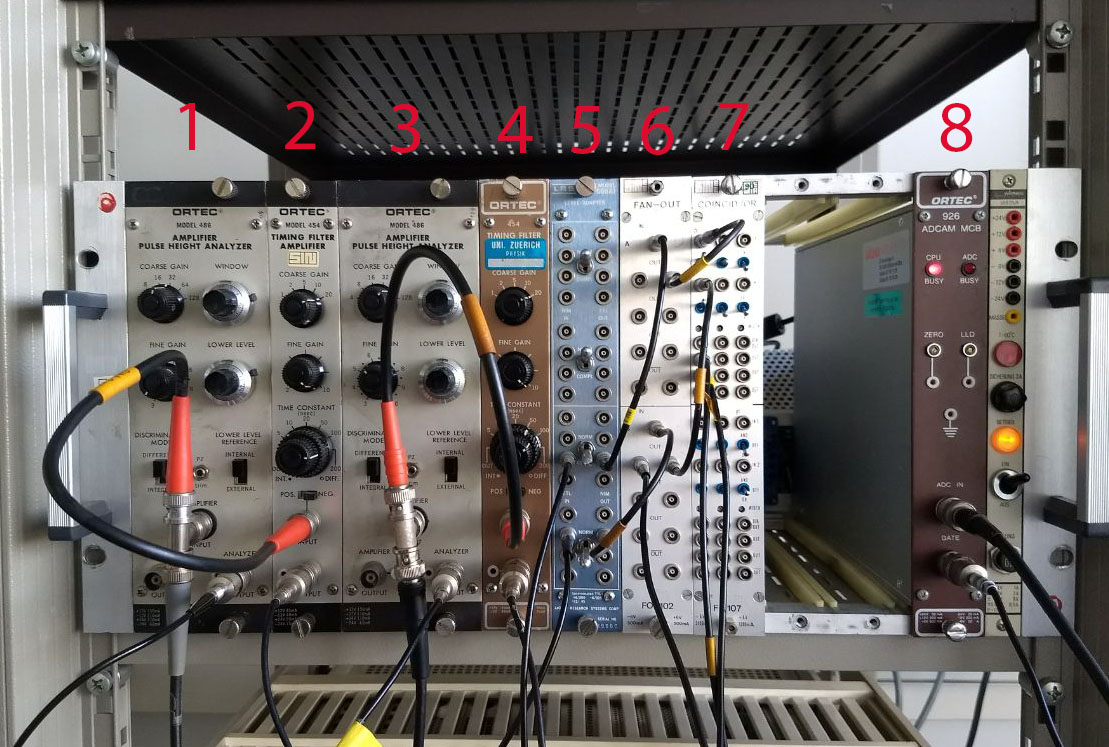
\includegraphics[scale=0.3]{Rack1-beschriftet.jpg}
\caption[Electronics2]{Photograph of the actual modules during the experiment: 1)PHA of $D_l$, 2)TFA of $D_l$, 3)PHA of $D_s$, 4)TFA of $D_s$, 5)LA, 6)Fan-out, 7)Coincidence module, 8)MCA}
\label{fig:Electronics2}
		\end{figure}
		\begin{figure}[H]
\centering
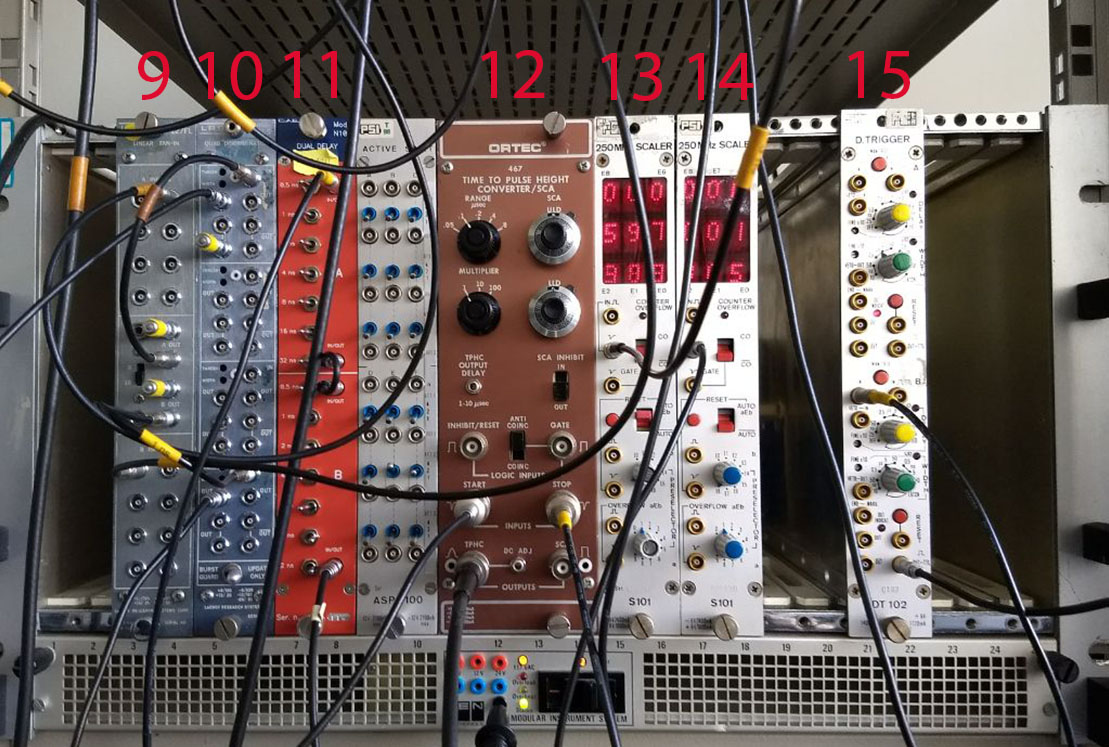
\includegraphics[scale=0.3]{Rack2-beschriftet.jpg}
\caption[Electronics3]{Photograph of the actual modules during the experiment: 9)Fan-out, 10)Discriminator, 11)Delay module, 12)TAC, 13)Scaler S1, 14)Scaler S2, 15)Delay Trigger}
\label{fig:Electronics3}
		\end{figure}

\section{Scintillation Counters and Photomultipliers}

The detectors used in this experiment are scintillation counters. They consist mainly of a scintillating material that is optically coupled to a photomultiplier tube. 

The molecules of a scintillating material (in this case NaI crystals doped with Thallium) become excited when radiation passes through and emit light during deexcitation (here with a wavelength of 410 nm). The intensity of this light emission depends linearly on the energy deposited. The light is then detected by a photomultiplier tube. [\ref{source:WilliamLeo}]
\begin{figure}[H]
\centering
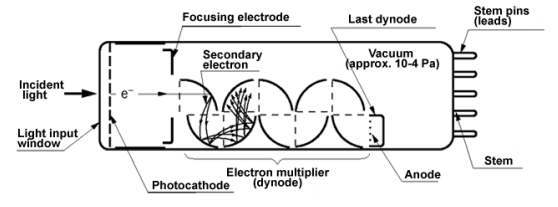
\includegraphics[scale=1]{Photomultiplier.png}
\caption[Photomultiplier]{Schematic illustration of a photomultiplier tube [\ref{source:WilliamLeo}]}
\label{fig:Photomultiplier}
		\end{figure}
The concept of a photomultiplier tube is illustrated in figure \ref{fig:Photomultiplier}. When light above a threshold energy hits the photocathode, an electron is ejected from this photosensitive material due to the photoelectric effect. The electron is accelerated towards an array of electrodes calles dynodes where the potential is increasing step by step at every dynode. When an electron strikes a dynode, more electrons are ejected from the material which are then accelerated towards the next dynode. Thus, the amount of electrons increases exponentially until they hit the anode in the end of the tube where they induce a measurable current that can be used as an analog signal. The cathode and dynode systems are assumed to be linear, meaning that the current signal at the output is directly proportional to the incoming amount of photons. [\ref{source:WilliamLeo}]

\chapter{Energy Spectrum} \label{sec:EnergySpectrum}

		Figure \ref{fig:EnergySpectra} shows the energy spectra measured at the two detectors correspondingly where the horizontal axis has been rescaled. The original scale can be found in figure \ref{fig:EnergyRaw} in the appendix, where the number of events was merely a function of ADC-channels. The two sharp peaks in the right half of the plot could be easily identified as the typical $\gamma$-decay absorption lines. Their corresponding energy values of $E_{\gamma,1}$ = 1172 keV and $E_{\gamma}$ = 1332 keV are well known in the literature and were used for the energy calibration that made the rescaling to energy units possible.	
		\begin{figure}[H]
\centering
\includegraphics[scale=0.3]{EnergySpectra.png}
\caption[EnergySpectra]{Energy spectra of each detector with tagged $\gamma$-ray absorption lines and typical detection byproducts}
\label{fig:EnergySpectra}
	\end{figure}	
		In addition to the two sharp gamma ray peaks, there is a typical Compton continuum visible on the left. The Compton edge can be obtained as follows [\ref{source:GlennKnoll}]
	\begin{equation}
E_{CE} = E_{\gamma} \cdot \left(1 - \frac{1}{1+2 E_{\gamma}/m_ec^2} \right).
\end{equation}
		This yields a value of $E_{CE,1}$ = 963 keV for the first $\gamma$-ray and $E_{CE,2}$ = 1118 keV for the second $\gamma$-ray. The first Compton edge is clearly visible in the plots while the second one coincides with the finite width of the first $\gamma$-ray line. Thus, it is clear that the Compton continuum does not vanish completely after the first edge.

		There is also an additional peak visible in both plots at around 200 keV in the case of the small detector and 150 keV for the large one. This is a very common effect that can be traced back to backscattering which originates from $\gamma$-rays that have Compton scattered in the material surrounding the detector material before being detected. In the literature, this peak is said to be expected at around 200 keV, which is in very good agreement with the measurement. It also makes sense that this peak is not the same for both detectors, since they are not identical models.

\chapter{Measurement Log}
For each angle in the range of $60^{\circ}$ to $180^{\circ}$ with steps of $15^{\circ}$ we took three 20 minute measurements: The number of coincident events measured with the software Maestro $r_m$, the number of coincident events measured by one of the scalers $r_s$, and the total number of events measured by the fixed detectors $r_{tot}$. The results of these measurements for each angle are listed in table \ref{tab:measurement}. 
%
\begin{table}[H]\label{tab:measurement}
\begin{center}
\begin{tabular}{lllll}
Angle $\theta$ [$^{\circ}$] & $r_{m}$ [Hz] & $r_{s}$ [Hz] & $r_{tot}$ [Hz]\\
\hline
60 	& 3.54 & 4.34 & 1470\\
75 	& 3.35 & 4.09 & 1469\\
90 	& 3.33 & 4.12 & 1469\\
105 	& 3.39 & 4.16 & 1468\\
120	& 3.44 & 4.20 & 1464\\
135	& 3.52 & 4.29 & 1464\\
150	& 3.60 & 4.35 & 1468\\
165	& 3.57 & 4.35 & 1466\\
180	& 3.67 & 4.31 & 1453\\ 
\end{tabular}
\caption{Measurement results}
\label{tab:measurement}
\end{center}
\end{table}
%
The software Maestro gave us not only the number of coincident events as listed in the table above, but the number of events for 8191 ADC channels. As an example, the histogram for $\theta = 90^{\circ}$ is shown in figure \ref{fig:histogramraw}, the rest can be found in the appendix on page \pageref{app:histogramraw}.
%
\begin{figure}[H]
\centering
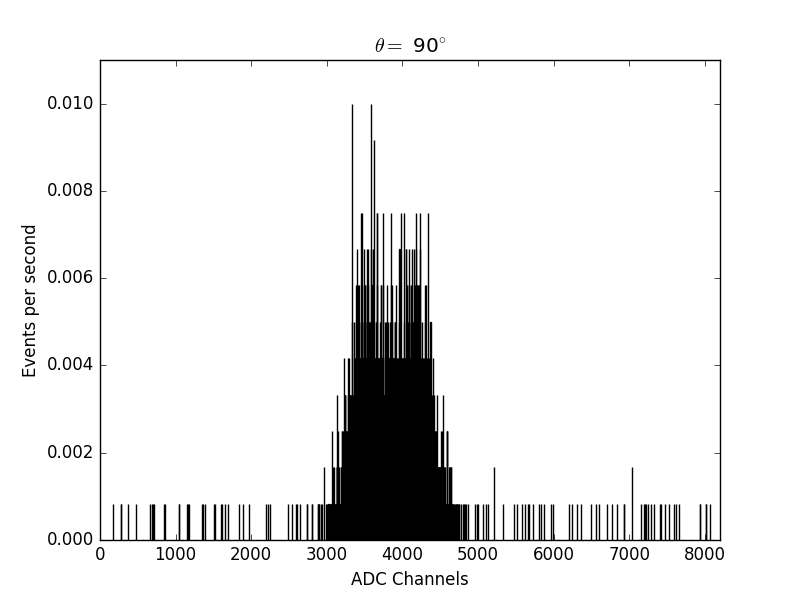
\includegraphics[scale=0.65]{90degraw.png}
\caption[Histogram]{Histogram with ADC channels for $\theta = 90^{\circ}$}
\label{fig:histogramraw}
\end{figure}
%



\chapter{Data Analysis}

\section{Time Calibration} \label{sec:TimeCal}

		Equivalently to the energy calibration in section [\ref{sec:EnergySpectrum}], the MCA transmitted the number of events as a function of the corresponding channel to the computer. In order to convert the channel number to the corresponding physical time delay, a time calibration measurement has been performed. This consisted of splitting the signal of one of the detectors and then connecting one copy directly to the start-channel of the TAC and the other one to the stop-channel after passing the delay module first. The signal that the TAC induces for various delay settings in the MCA could then be directly observed in the computer. Data was collected and saved for five different delay settings, which can be seen in figure \ref{fig:TimeCal1}.
		\begin{figure}[H]
\centering
\includegraphics[scale=0.5]{TimeCalibration1.png}
\caption[TimeCalibration1]{Time calibration measurement where each line corresponds to a known delay time}
\label{fig:TimeCal1}
	\end{figure}
	From this, we could deduce which channel corresponds to which magnitude of delay. The channel number and their corresponding delay time were plotted and a linear fit through the data points could be performed (see figure \ref{fig:TimeCal2}), which yields the following rescaling function where $\hat{T}$ corresponds to the time-scale in [ns] and $\hat{C}$ to the channel-scale
	\begin{equation}
	\hat{T} = \hat{C} \cdot 0.0111 \mathrm{ns} + 5.2041 \mathrm{ns} 
	\end{equation}
	\begin{figure}[H]
\centering
\includegraphics[scale=0.39]{TimeCalibration2.png}
\caption[TimeCalibration2]{Linear fit through the corresponding delay-channel-points}
\label{fig:TimeCal2}
	\end{figure}

\section{Gaussian Fit}

%Since each measurement lasted for 20 minutes, the statistical errors on these measurements should be negligible. To check this assumption, we calculated the statistical uncertainty on the measurement made by S1). Since S1 was counting the number of events registered by the fixed detector, we would expect it to measure the same value in each of the $n$ measuring periods. The relative statistical uncertainty can thus be calculated by
%%
%\begin{align}
%\frac{\Delta r}{\overline{r}} = \frac{1}{\overline{r}}\sqrt{\frac{\sum_i (r_i - \overline{r})^2}{n(n-1)}} \approx 0.1\%
%\end{align}
%%
%Assuming the same statistical uncertainty on the Maestro data $r_m$ which consists of values in a range of $5\%$ around their mean, this statistical uncertainty can indeed be neglected.
%
%
We started by rescaling the x-axis from ADC channels to time (see section \ref{sec:TimeCal}). To make sure there are enough counts per bin we had to rebin the data. We merged 20 bins to one, giving us a time resolution of $0.22\,$ns. We then used the $\chi^2$-method to fit a Gaussian function on each histogram, taking into account an uncertainty on each bin of 
%
\begin{align}
\Delta_{bin} = \sqrt{n_{bin}}
\end{align}

Figure \ref{fig:hist120} shows the histogram with gaussian fit for the angle $\theta = 90^{\circ}$. The rest of the histograms can be found in the appendix on page \pageref{app:histogram}.
%
\begin{figure}[H]
\centering
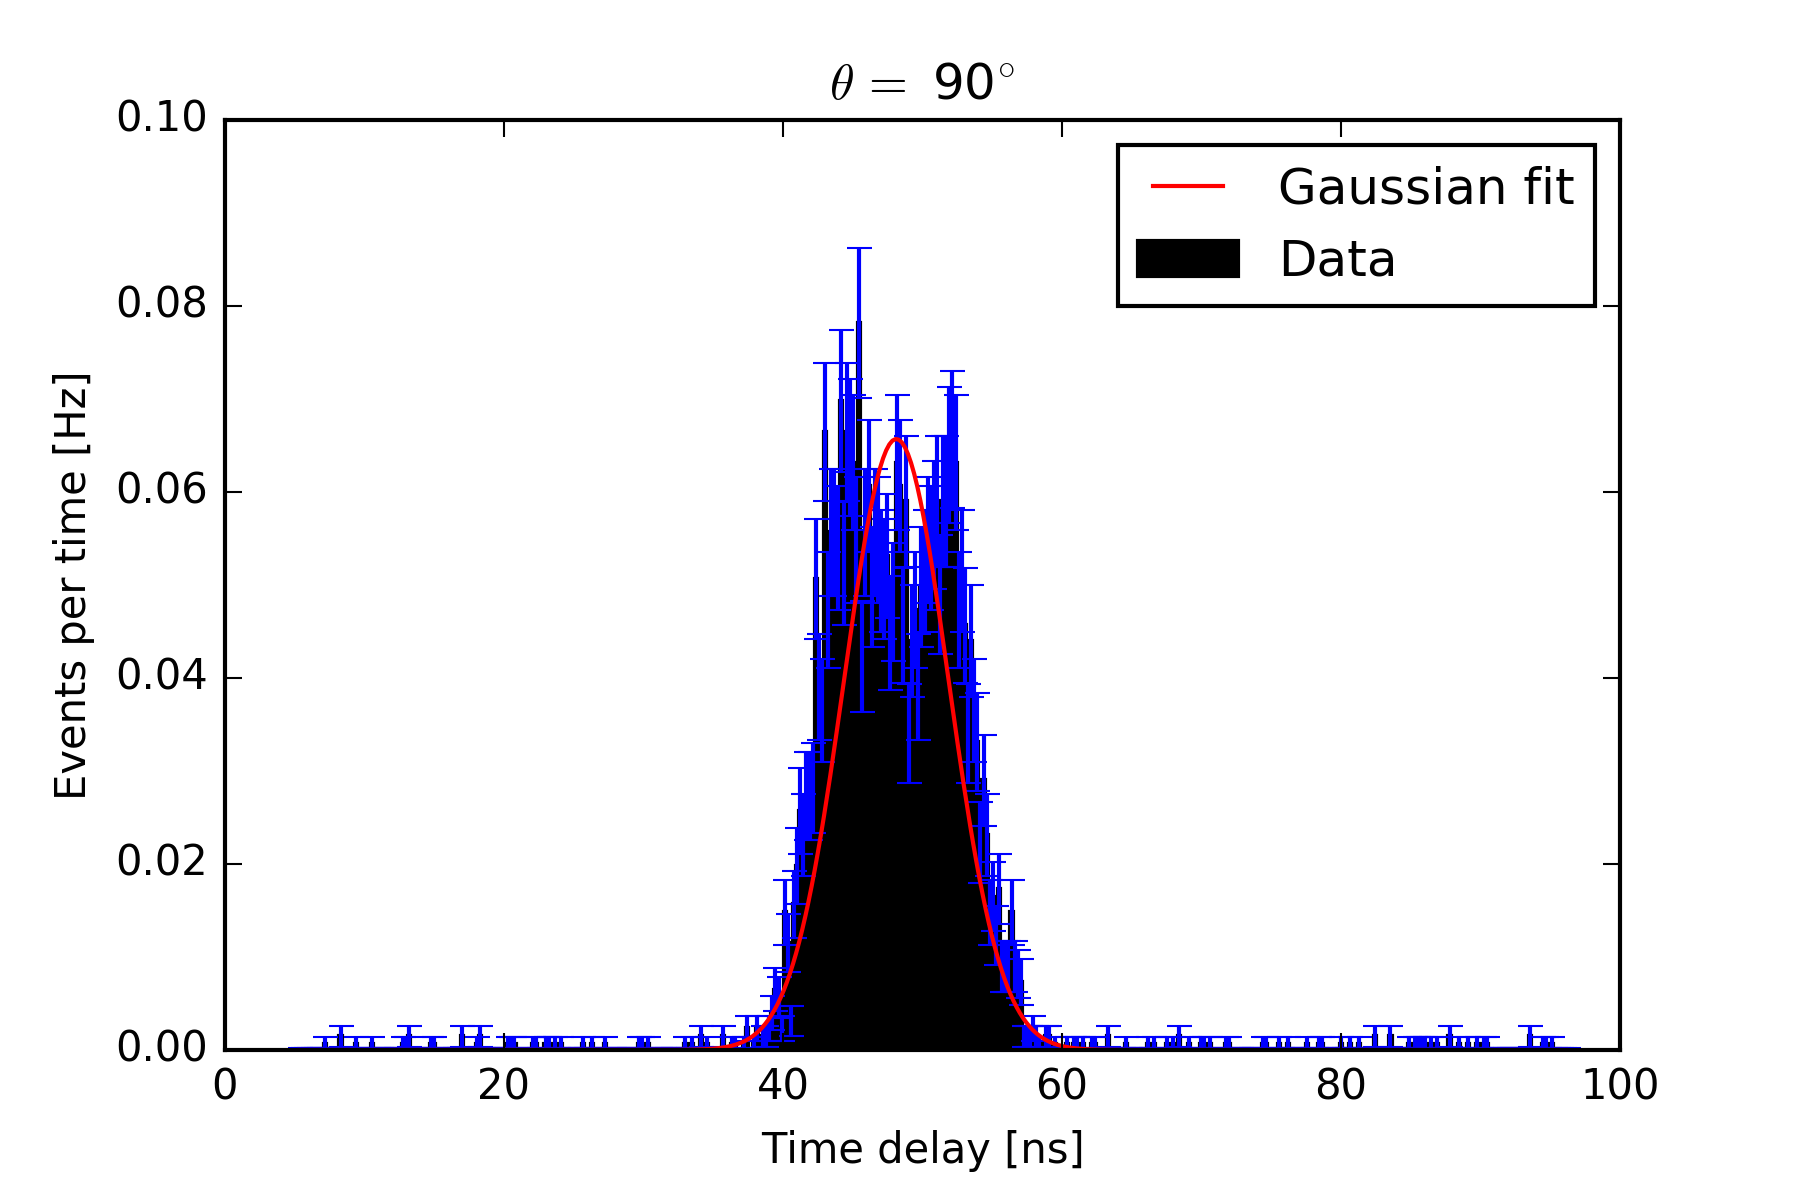
\includegraphics[scale=0.65]{90deg.png}
\caption[Histogram]{Histogram with gaussian fit for angle $\theta = 90^{\circ}$}
\label{fig:hist120}
\end{figure}
%
We noticed that the measured data does not show a single peak at the set delay time, but instead two peaks slightly below and above. A reason for this might be the poor stability of the trigger settings in the discriminator. In a next step, we subtracted the background from the data. In order to estimate the background, we took the average of the bins in a range of [$3\sigma$, $4\sigma$] on both sides of the mean $\mu$. Then we subtracted this average from each bin in the histogram. We then summed all the bins in a range of [$\mu$-3$\sigma$, $\mu$+3$\sigma$] in the histogram to get the number of coincident events per second $r_c$ for each angle. The statistical uncertainty was estimated by taking the square-root of the number of counts and normalizing it accordingly. Table \ref{tab:nevents} shows the result for each angle compared to the number of coincident events per second $r_{s}$ as measured by the scaler.
%
\begin{table}[H]
\begin{center}
\begin{tabular}{llll}
Angle $\theta$ [$^{\circ}$] & $r_{c}$ [Hz] & $r_{s}$ [Hz]\\
\hline
60 	& 3.42 $\pm$ 0.05 & 4.34\\
  75 	& 3.24 $\pm$ 0.05 & 4.09\\
  90 	& 3.23 $\pm$ 0.05 & 4.12\\
105 	& 3.30 $\pm$ 0.05 & 4.16\\
120	& 3.36 $\pm$ 0.05 & 4.20\\
135	& 3.42 $\pm$ 0.05 & 4.29\\
150	& 3.50 $\pm$ 0.05 & 4.35\\
165	& 3.47 $\pm$ 0.05 & 4.35\\
180	& 3.54 $\pm$ 0.05 & 4.31\\ 
\end{tabular}
\caption{Rate for each angle}
\label{tab:nevents}
\end{center}
\end{table}
%

\section{Angular Correlation Function} \label{sec:DataAnalysis}

In order to be able to compare this data to the predicted value, we normalized the data to $r_{c}(\theta=90^{\circ})$. Then we used the $\chi^2$-method to fit a function in the form of equation \ref{eq:distribution} to the data points (figure \ref{fig:distribution}).
\begin{equation} \label{eq:distribution}
W(\theta) = a_0 + a_1 \cos^2 \theta + a_2 \cos^4 \theta
\end{equation}
This corresponds to formula \ref{eq:Ang1} with leaving $a_0$ as a free parameter instead of constraining it to exactly 1.
%
\begin{figure}[H]
\centering
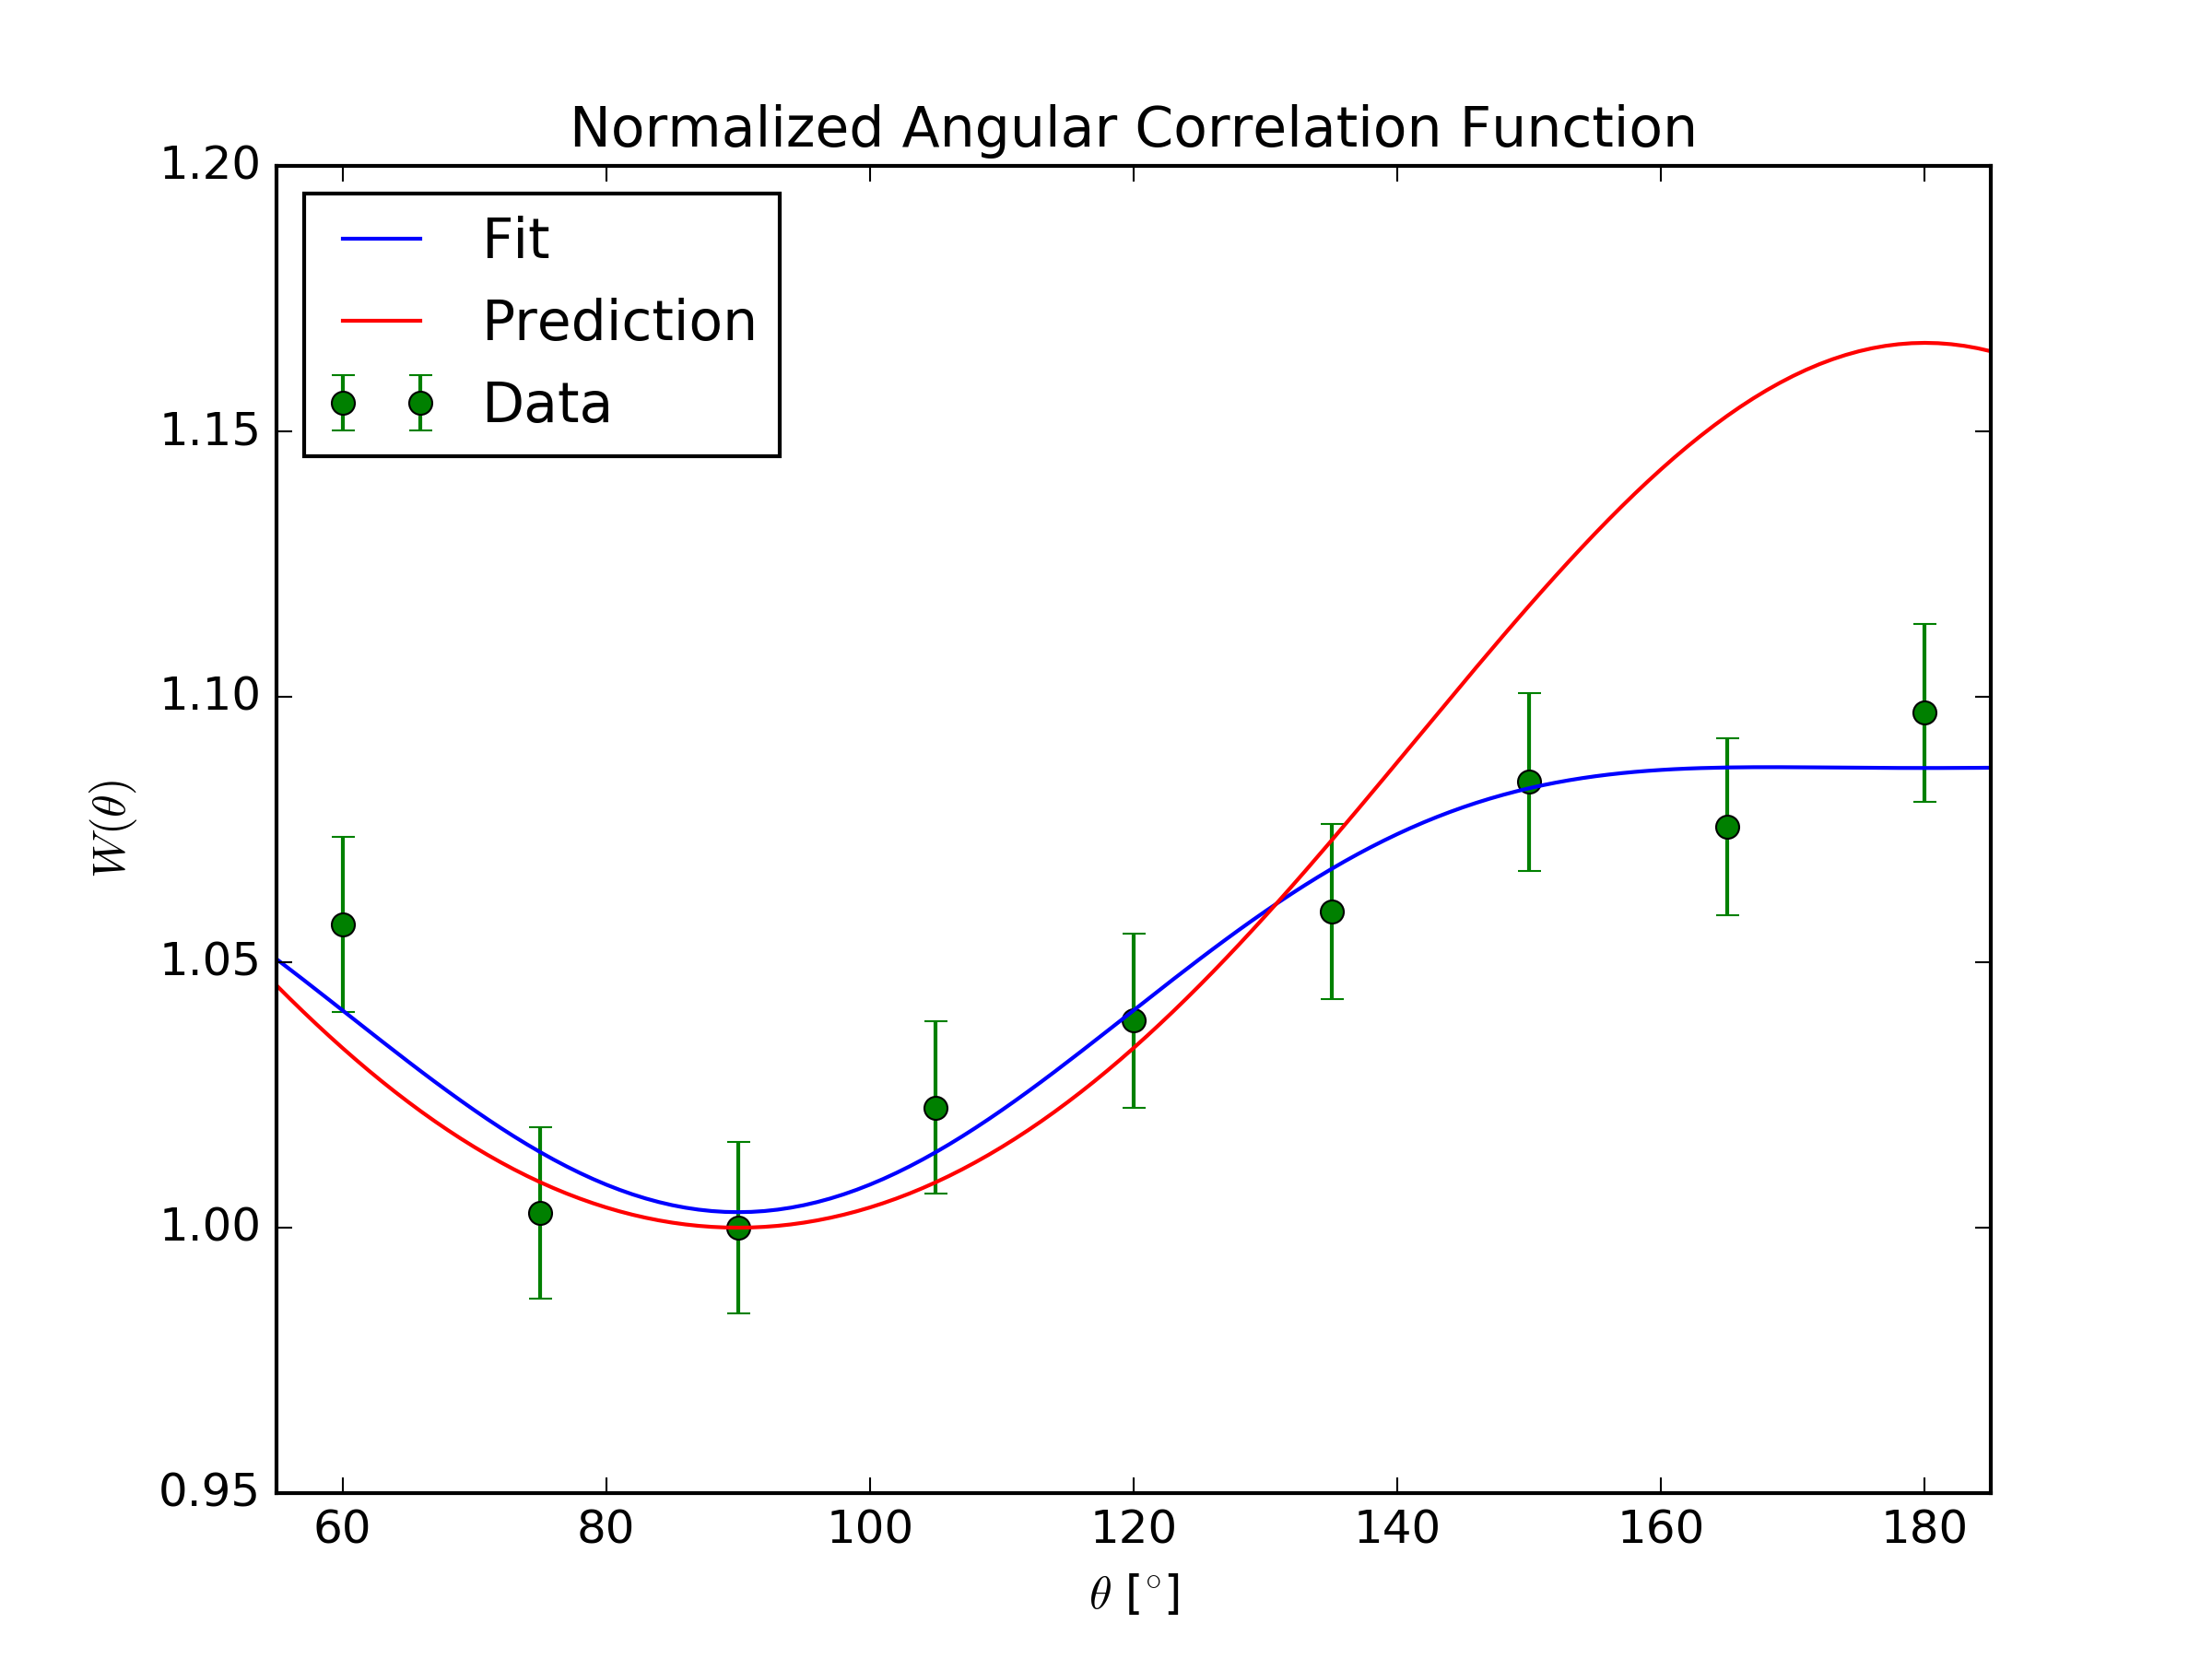
\includegraphics[scale=0.65]{dist.png}
\caption[Distribution]{Normalized angular distribution}
\label{fig:distribution}
\end{figure}
%
For the coefficients $a_i$ we obtained:
%
\begin{align*}
a_0 &= 1.003 \pm 0.007\\
a_1 &= 0.175 \pm 0.044\\
a_2 &= -0.091 \pm 0.043\\
\end{align*}
%

\chapter{Conclusion}
\section{Results}

Comparing the results
%
\begin{align*}
a_0 &= 1.003 \pm 0.007\\
a_1 &= 0.175 \pm 0.044\\
a_2 &= -0.091 \pm 0.043\\
\end{align*}
%
derived in section \ref{sec:DataAnalysis} to the literature values [\ref{source:Hamilton}]
%
\begin{align*}
a_{0,lit} &= 1\\
a_{1,lit} &= 1/8 = 0.125\\
a_{2,lit} &= 1/24 \approx 0.042\\
\end{align*}
%
we see that $a_{0,lit}$ is clearly within the range while $a_{1,lit}$ is sligthly out of range. $a_{2,lit}$, on the other hand, is notably out of range. From figure \ref{fig:distribution} it is clearly visible that our measured data does not verify the prediction for angles starting at $\theta=135^{\circ}$. In the range of $\theta \in \left[60^{\circ},120^{\circ}\right]$ the measured data corresponds to the prediction.

\section{Discussion of Error Sources}

A closer look at the vertical axes in figure \ref{fig:EnergySpectra} yields that the larger detector detector around twice as many events as the smaller one, despite the adjustments in behalf of solid angle coverage. For a better measurement, it might be wise to use identical detector models at equal distances.

The scaler S2 merely measures the amount of approximately coincident events from both detectors. Using the 'time-branch', more information is provided. Namely, the overlay of the TAC-signal and the gate-input from the delay trigger add more nuance by providing a quantitative delay between allegedly coincident events. As expected, the number of events counted by S2 was significantly higher at every angel. Nevertheless, it supplied a cross-check in the sense that the sclaer values behave the same way as the ones obtained by the TAC-signal. This similarity verifies that the electronic modules act as expected.

A significant source of uncertainty might come from the poor stability of the trigger settings in the discriminator that let to the splitting of the expected gaussian distribution into two discrete peaks. In order to avoid such error, one would have to be more careful when adjusting the trigger in the future. Another way to deal with this problem would have been using a NIM signal again for the input of the discriminator.

In general, the measurement lacked a good degree of stability. A test run yielded that even slightly touching the cables could have an effect on the measurement. Not to mention the effect that the presence of the students and assistants might have had on the outcome. Thus we conclude that a more isolated setting could further improve the measurement.



\chapter{Appendix}

\section{Energy Spectrum}
%
\begin{figure}[H]
\centering
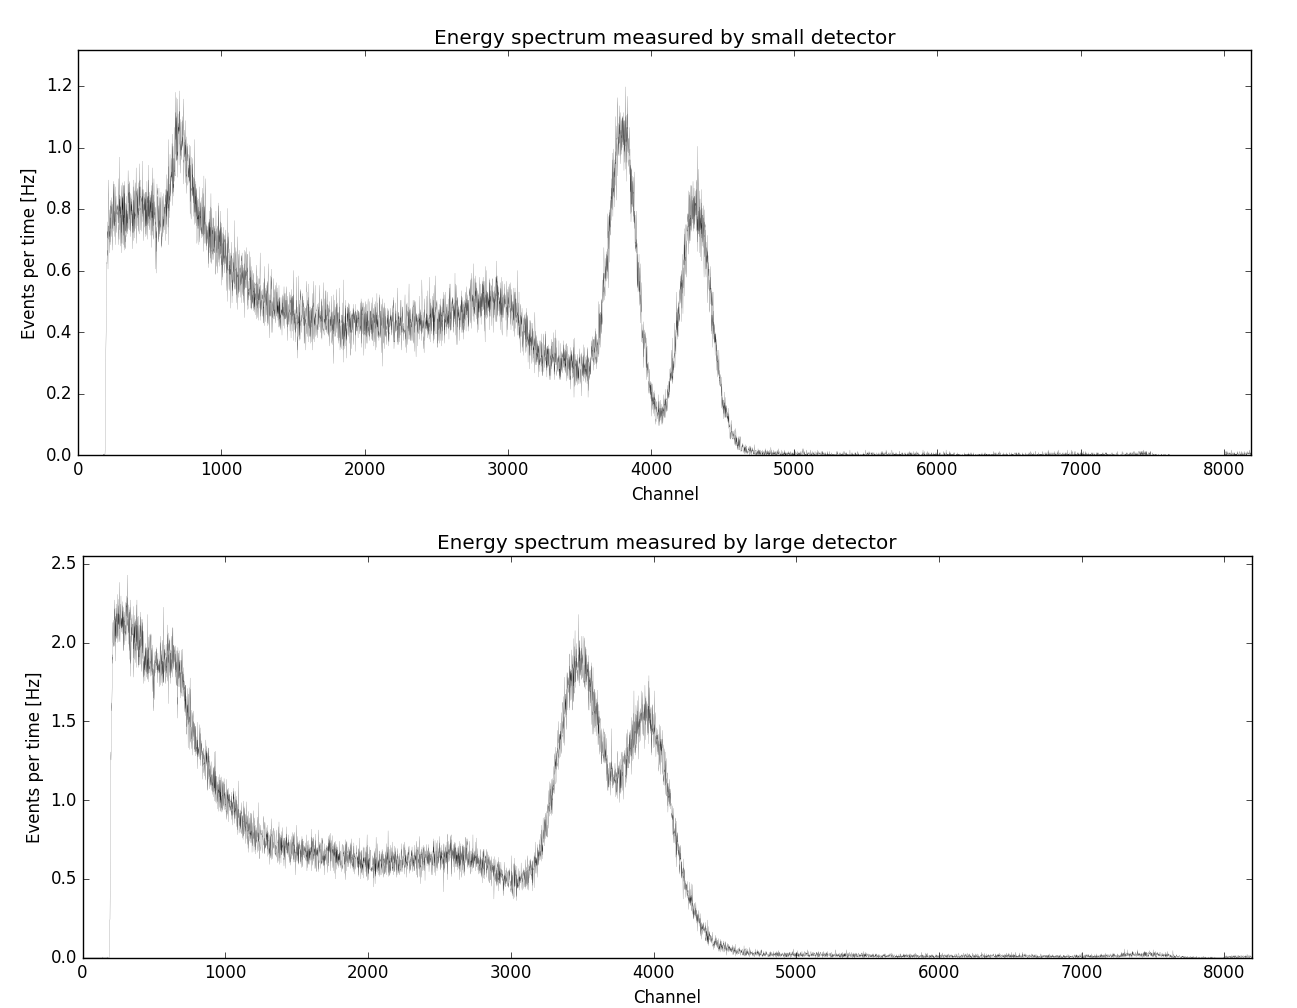
\includegraphics[scale=0.35]{EnergyRaw.png}
\caption[EnergyRaw]{Energy spectrum measured as a function of ADC channels}
\label{fig:EnergyRaw}
\end{figure}

\section{Measurement Log}\label{app:histogramraw}
%
\begin{figure}[H]
\centering
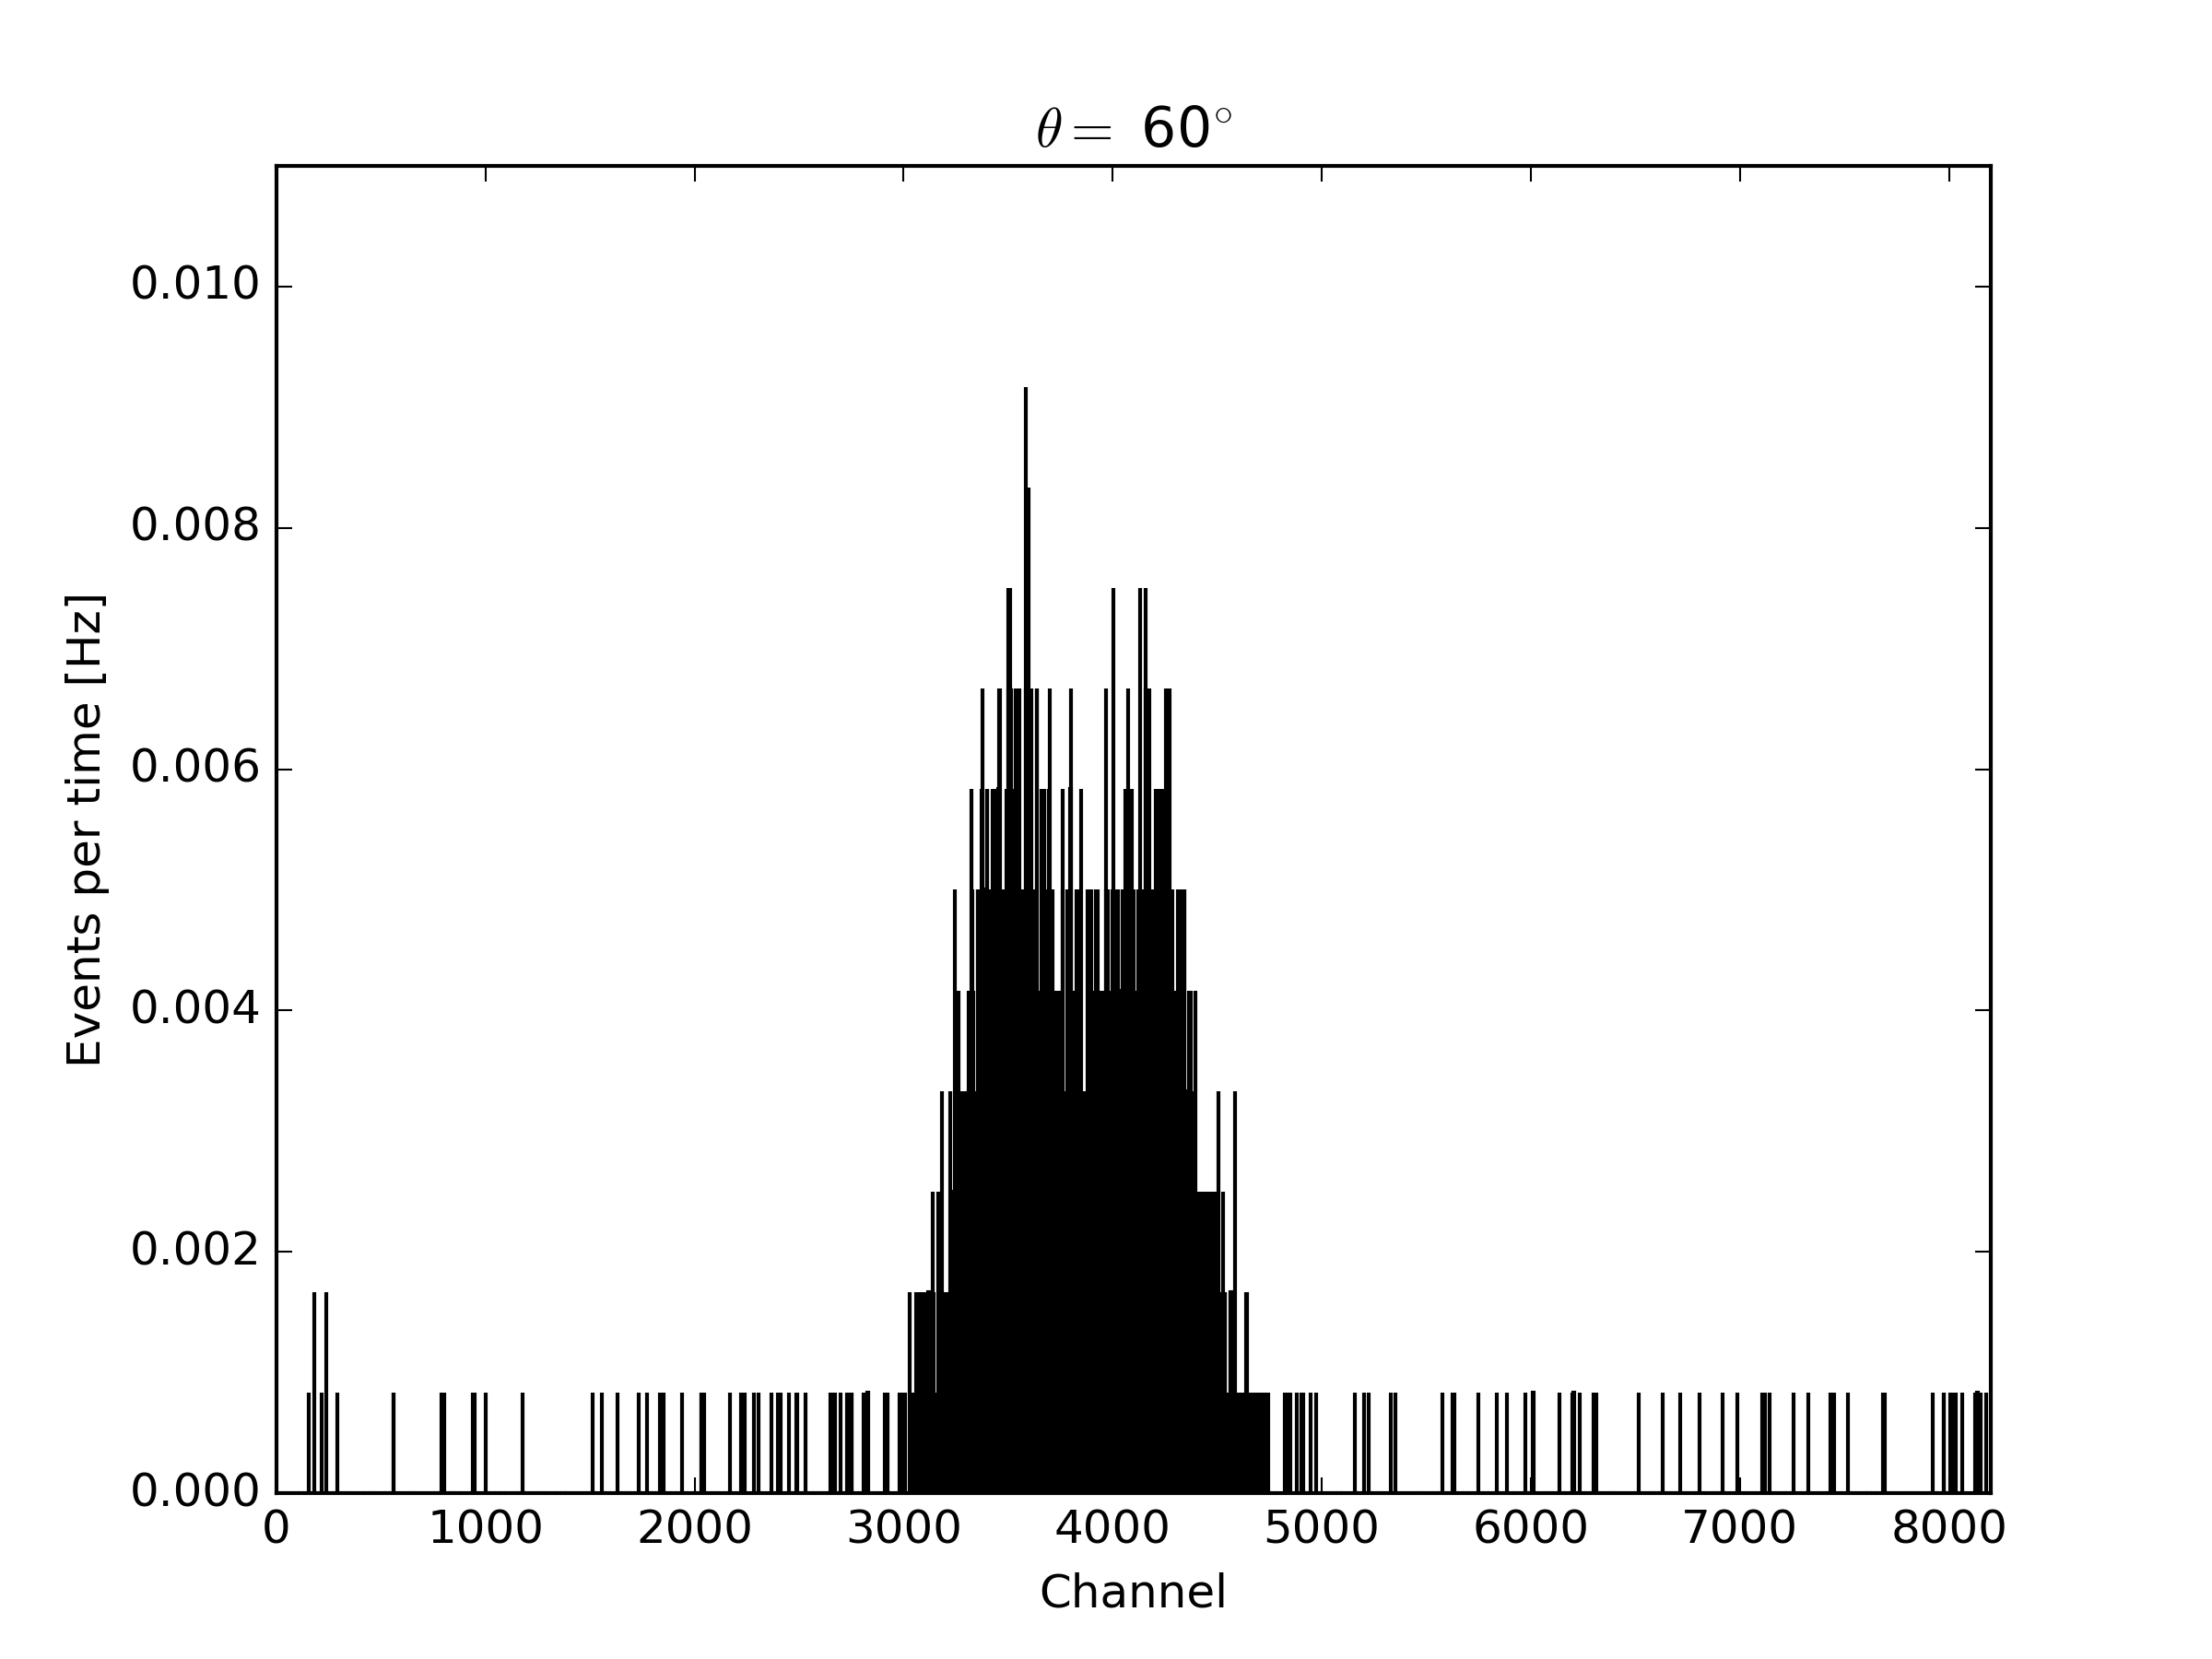
\includegraphics[width=0.33\textwidth]{60degraw.png}\hfill
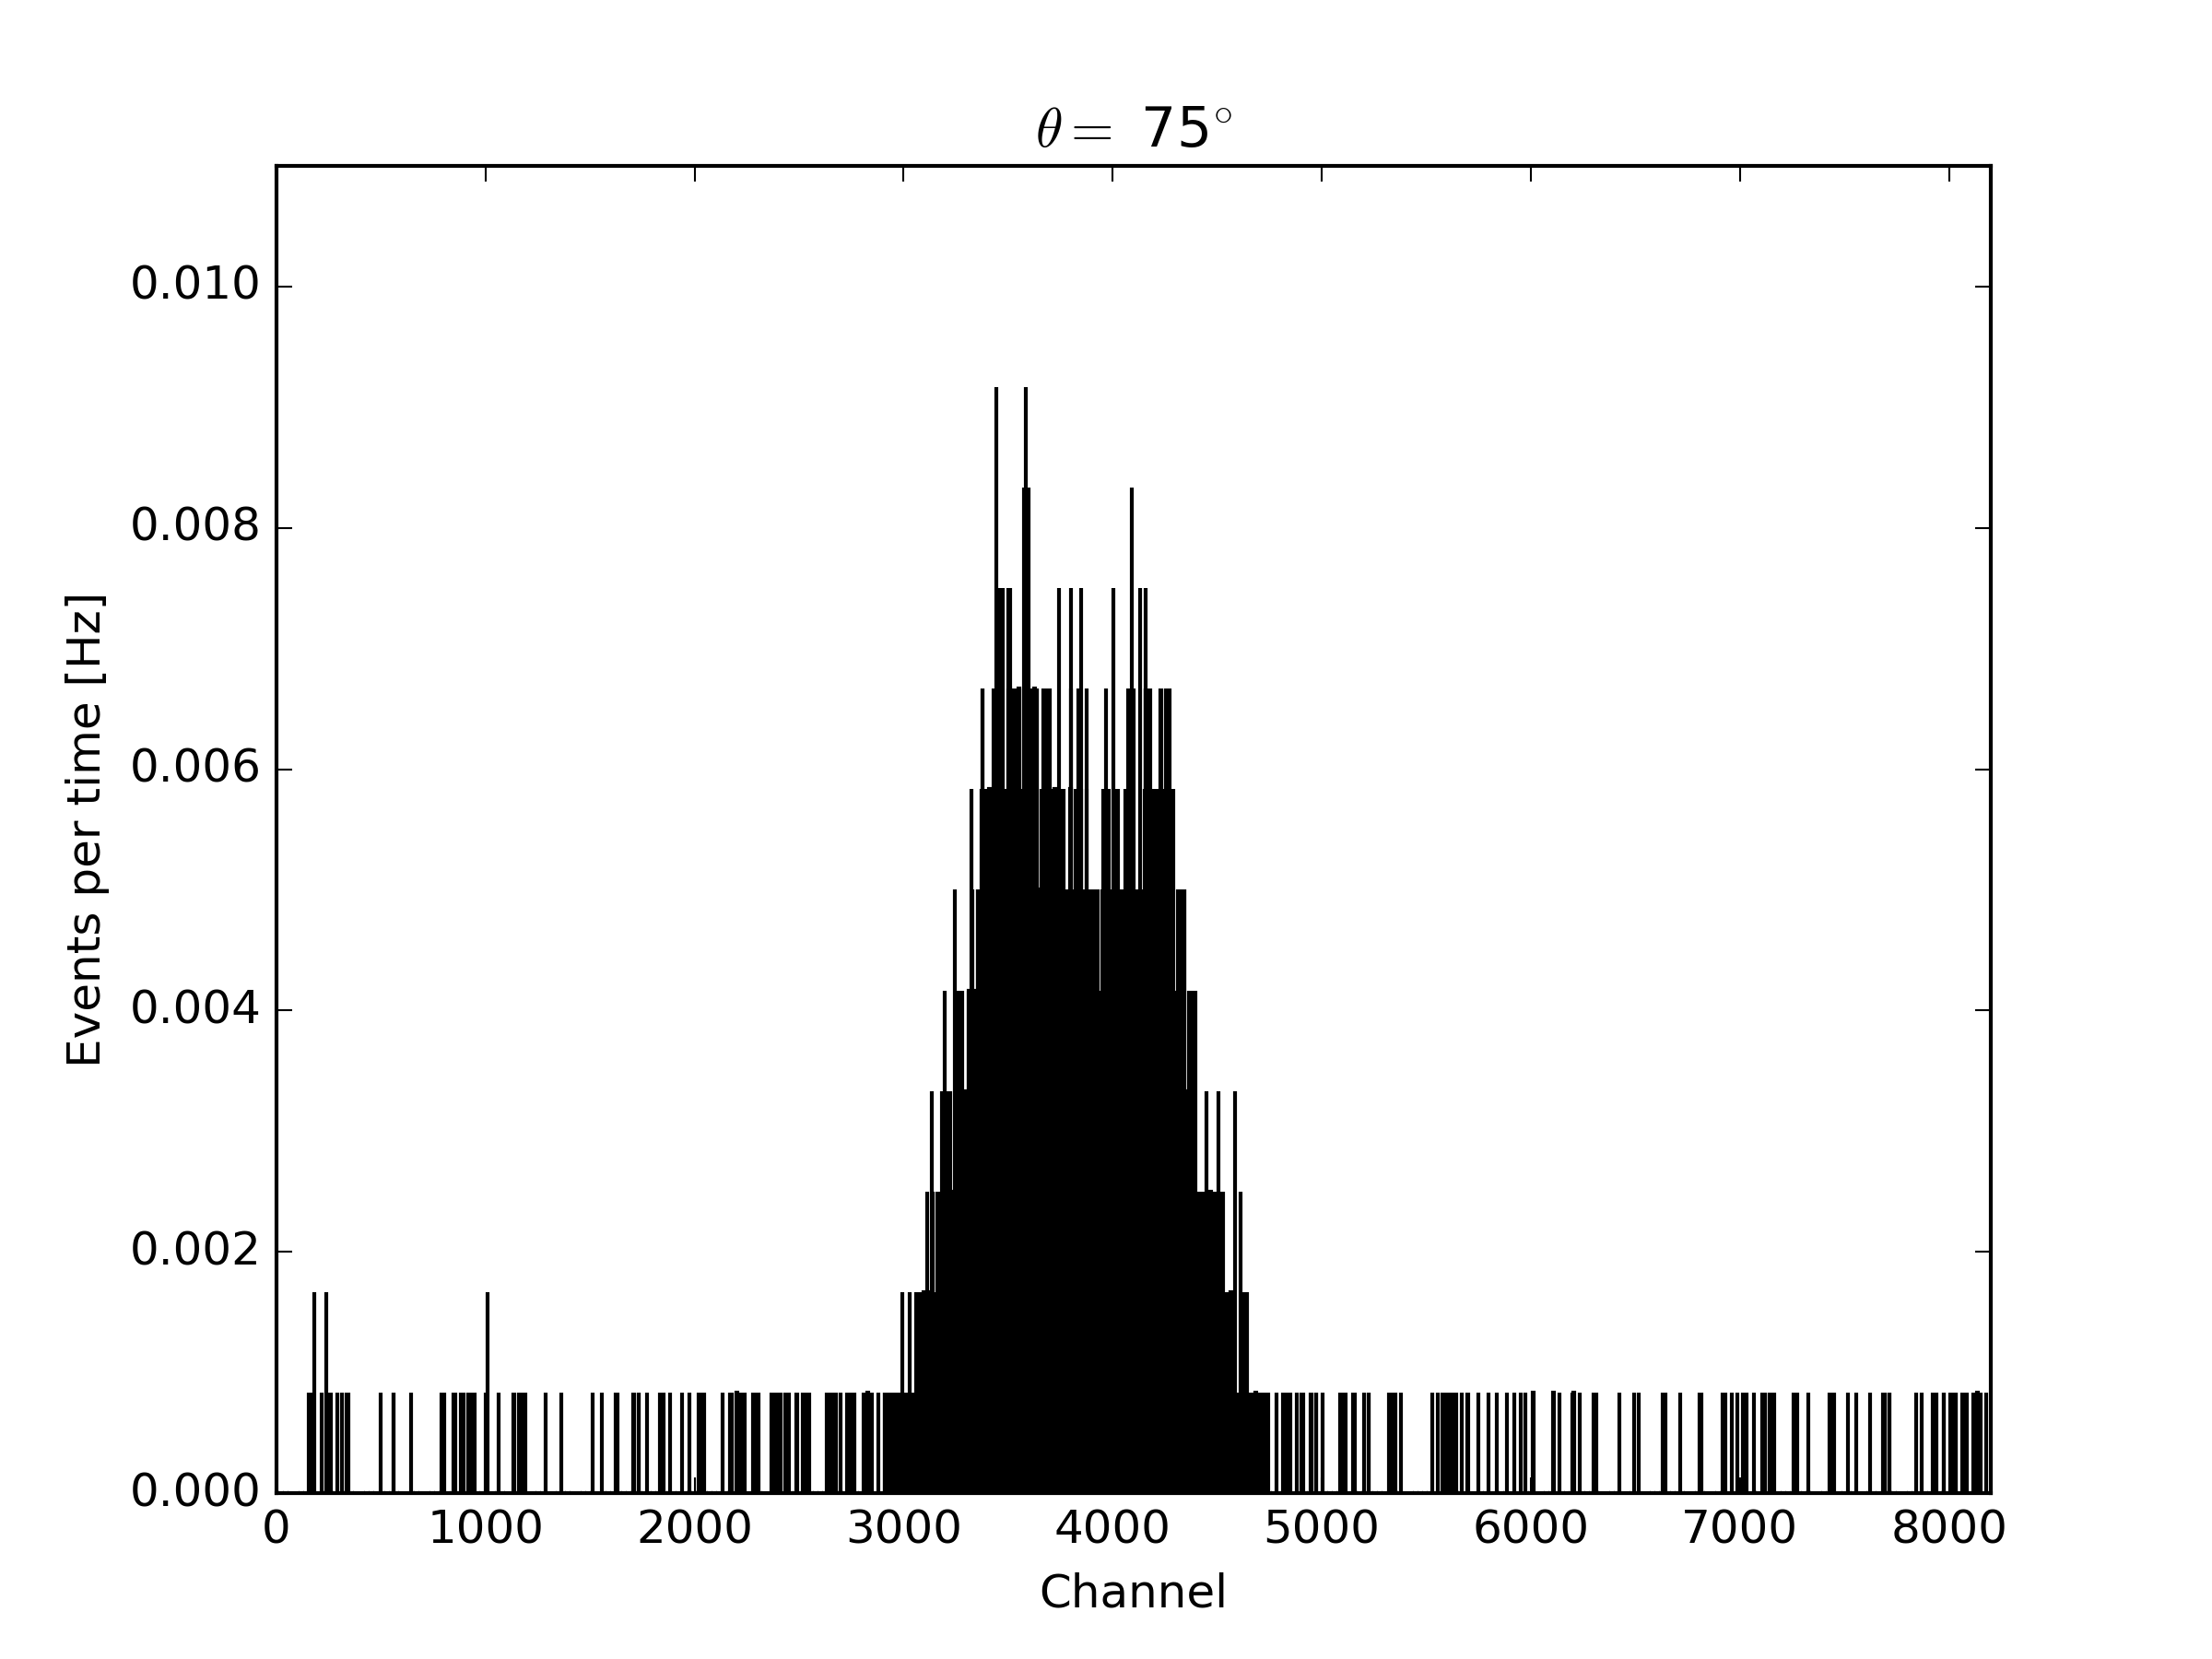
\includegraphics[width=0.33\textwidth]{75degraw.png}\hfill
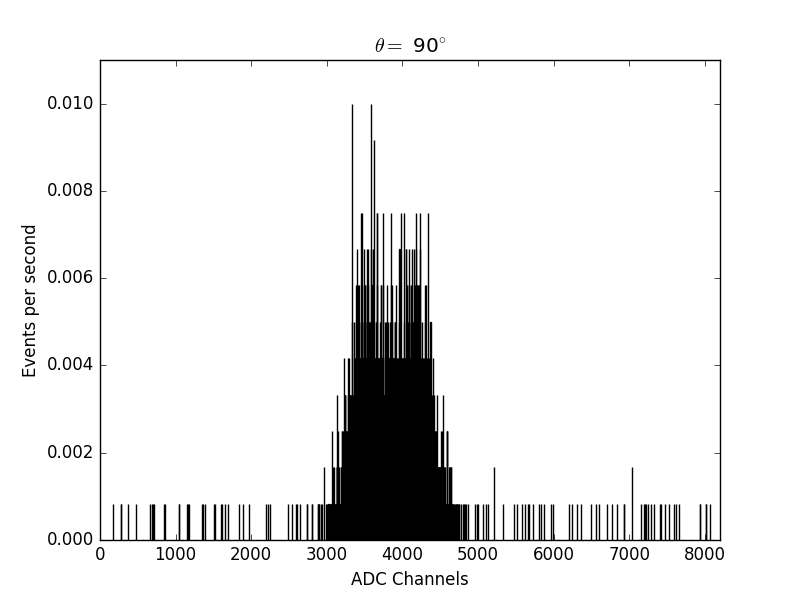
\includegraphics[width=0.33\textwidth]{90degraw.png}\\
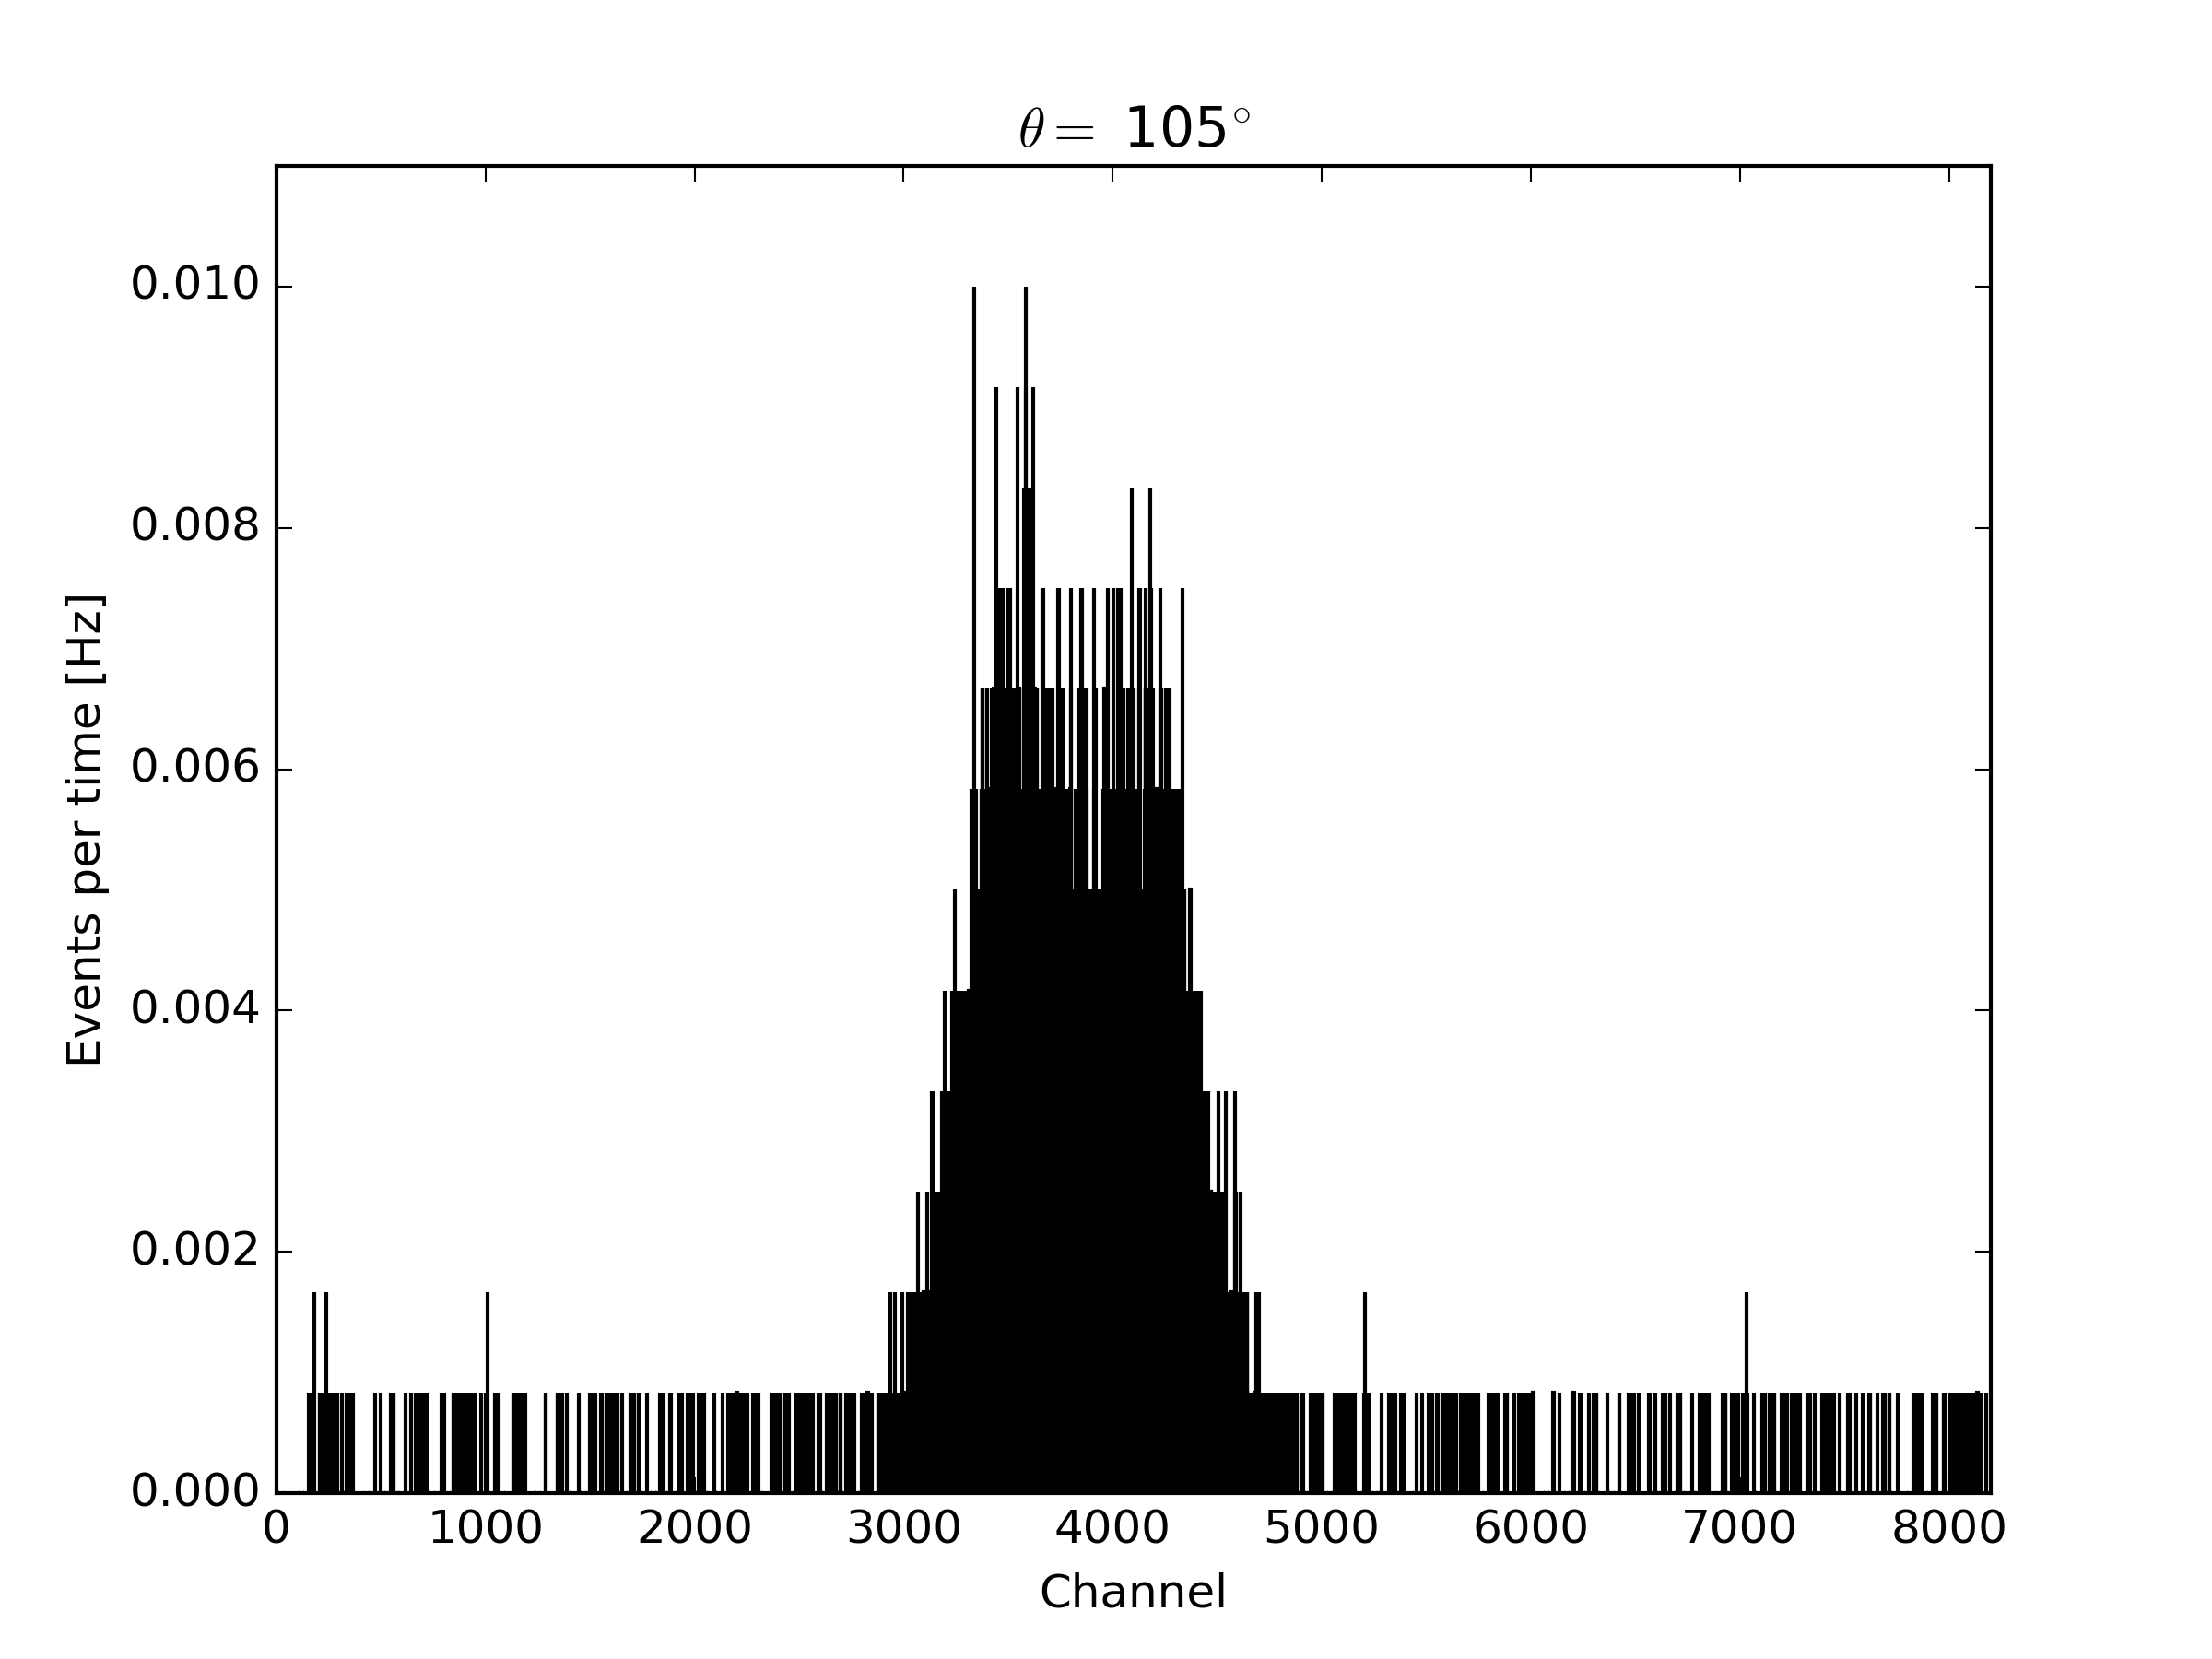
\includegraphics[width=0.33\textwidth]{105degraw.png}\hfill
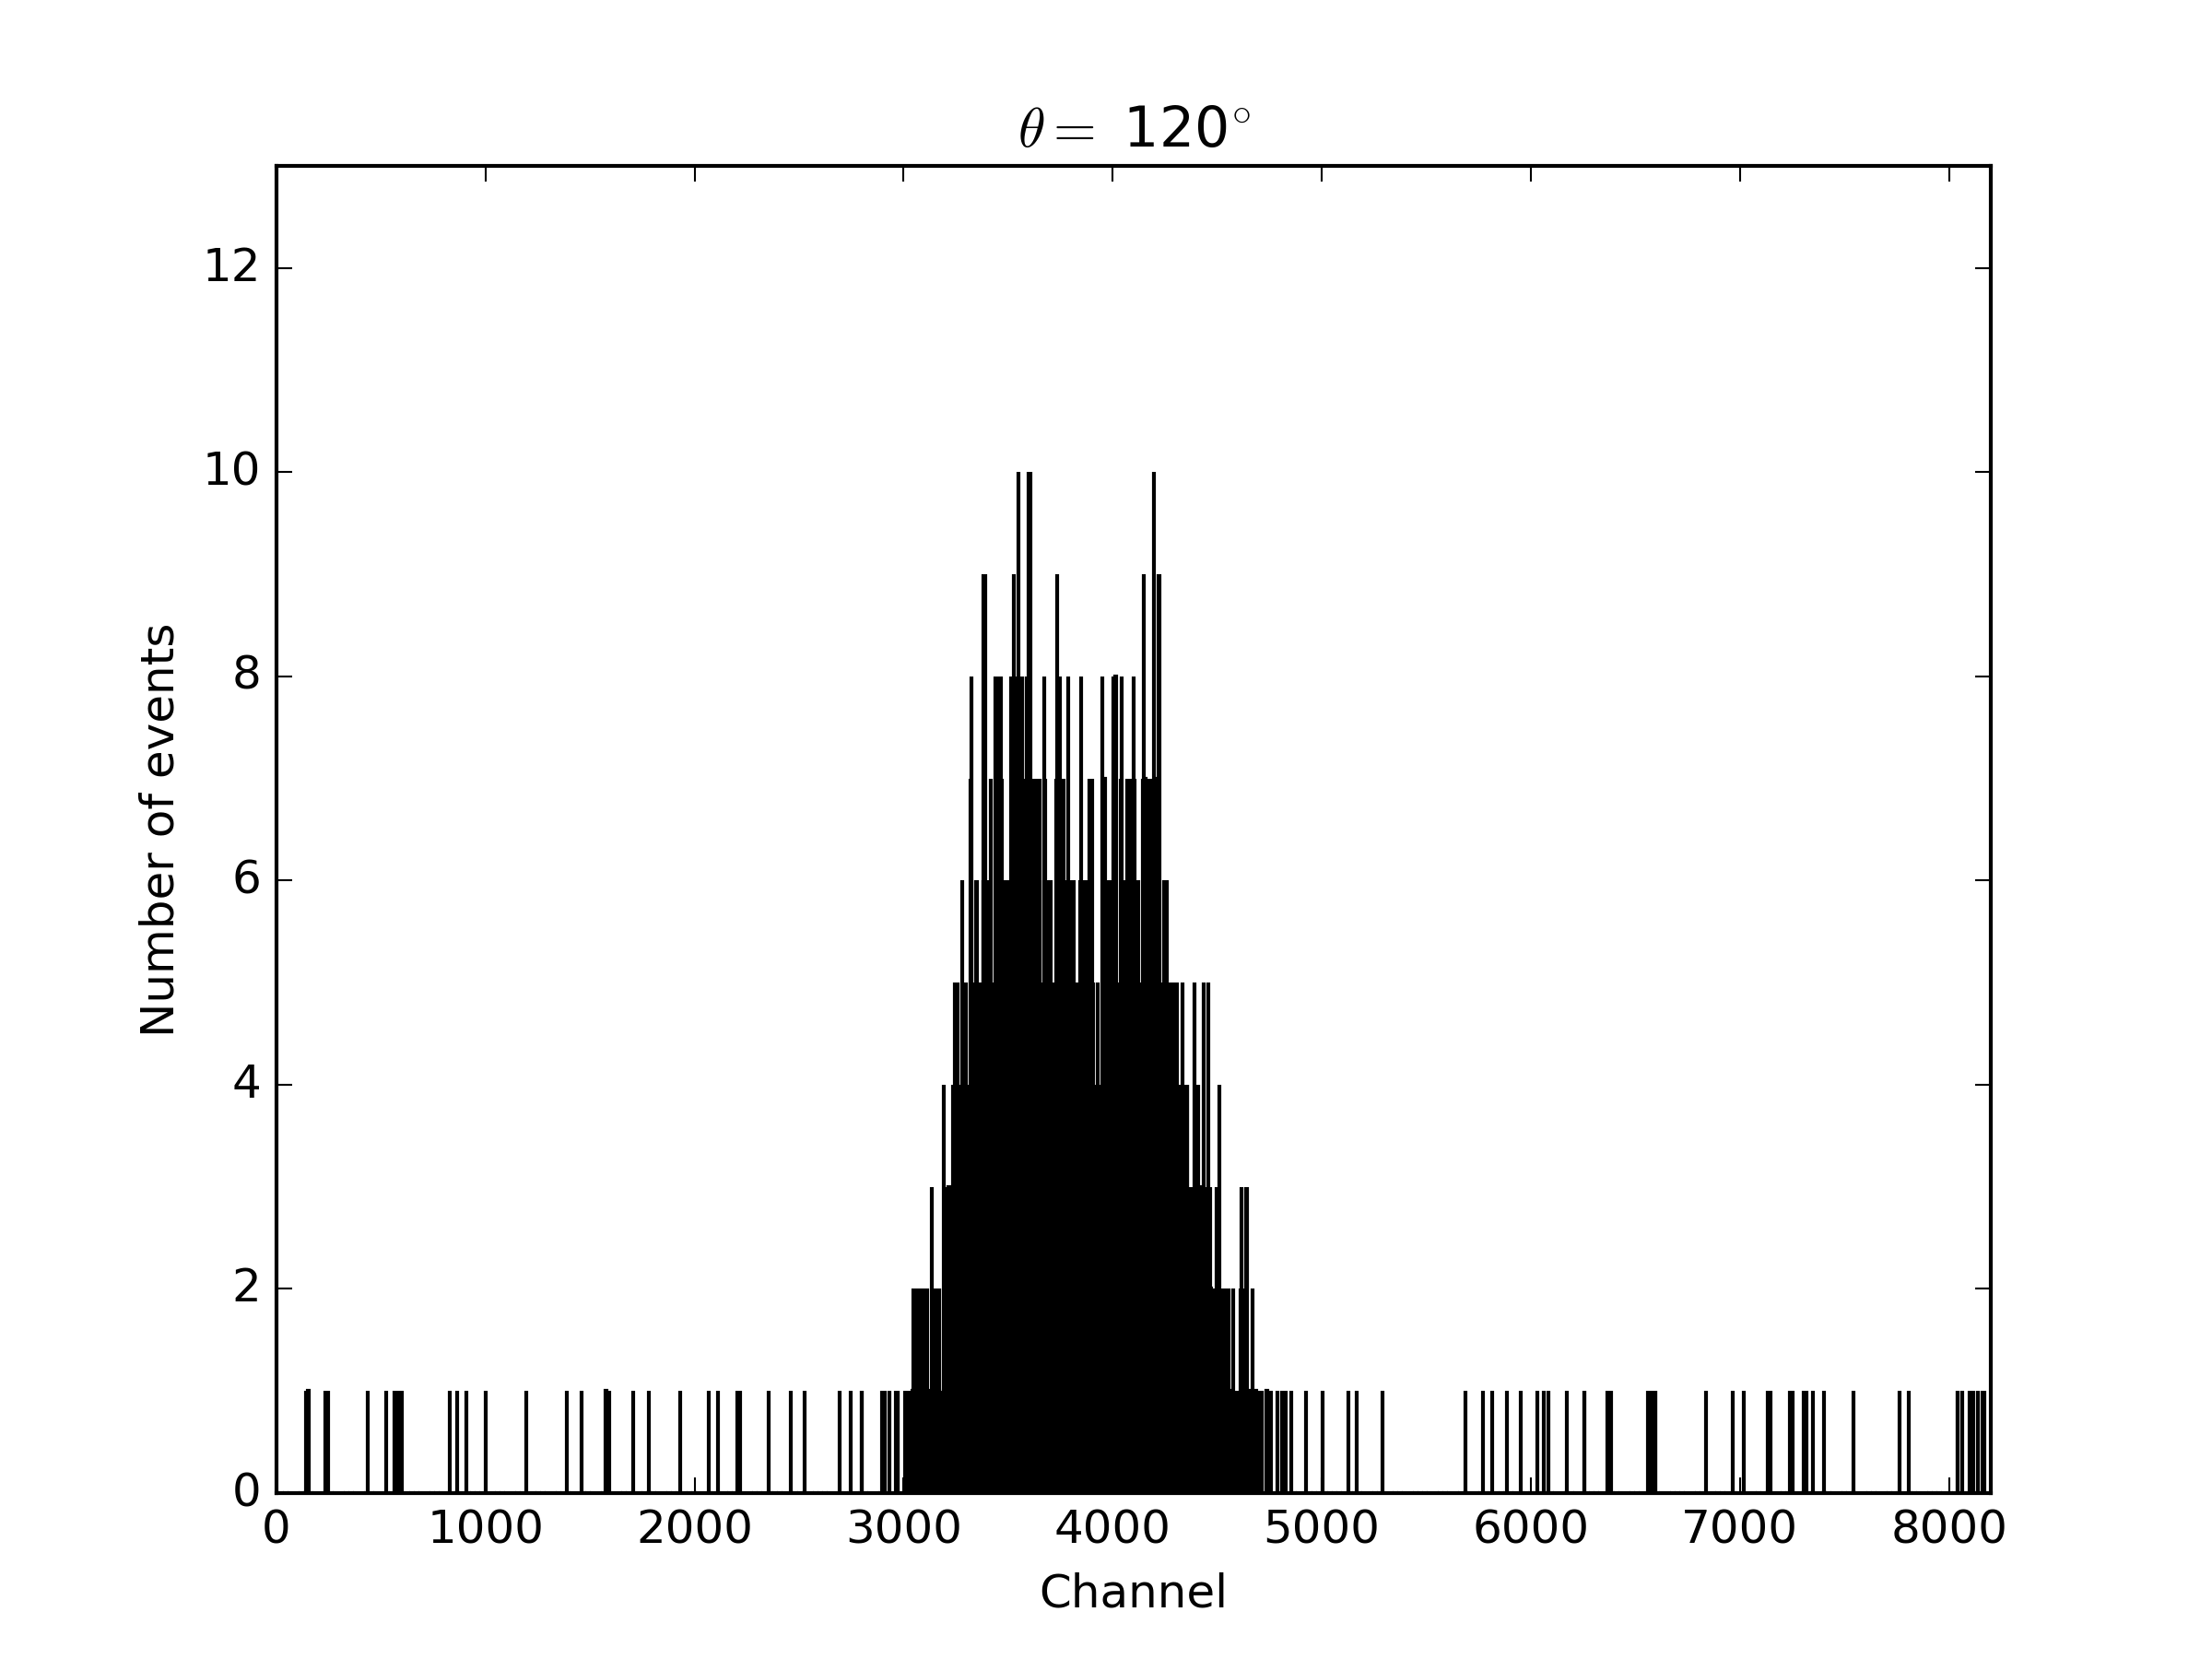
\includegraphics[width=0.33\textwidth]{120degraw.png}\hfill
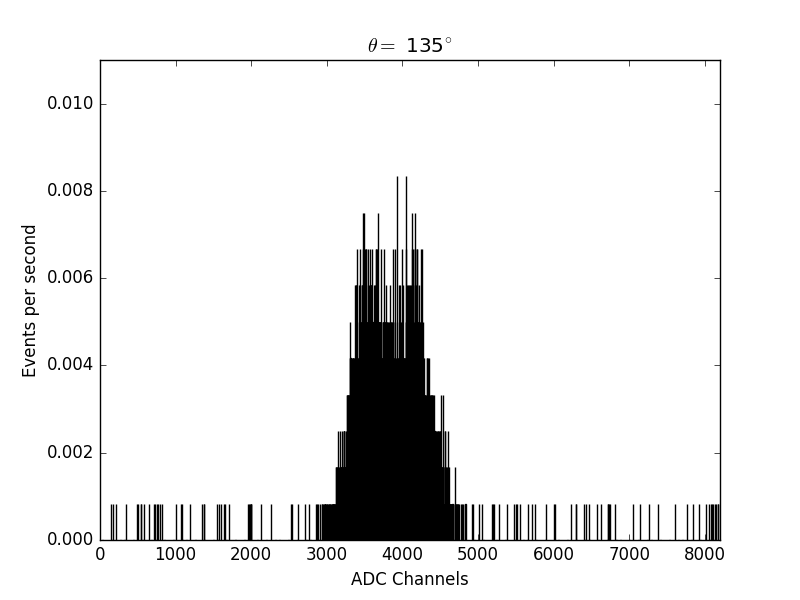
\includegraphics[width=0.33\textwidth]{135degraw.png}\\
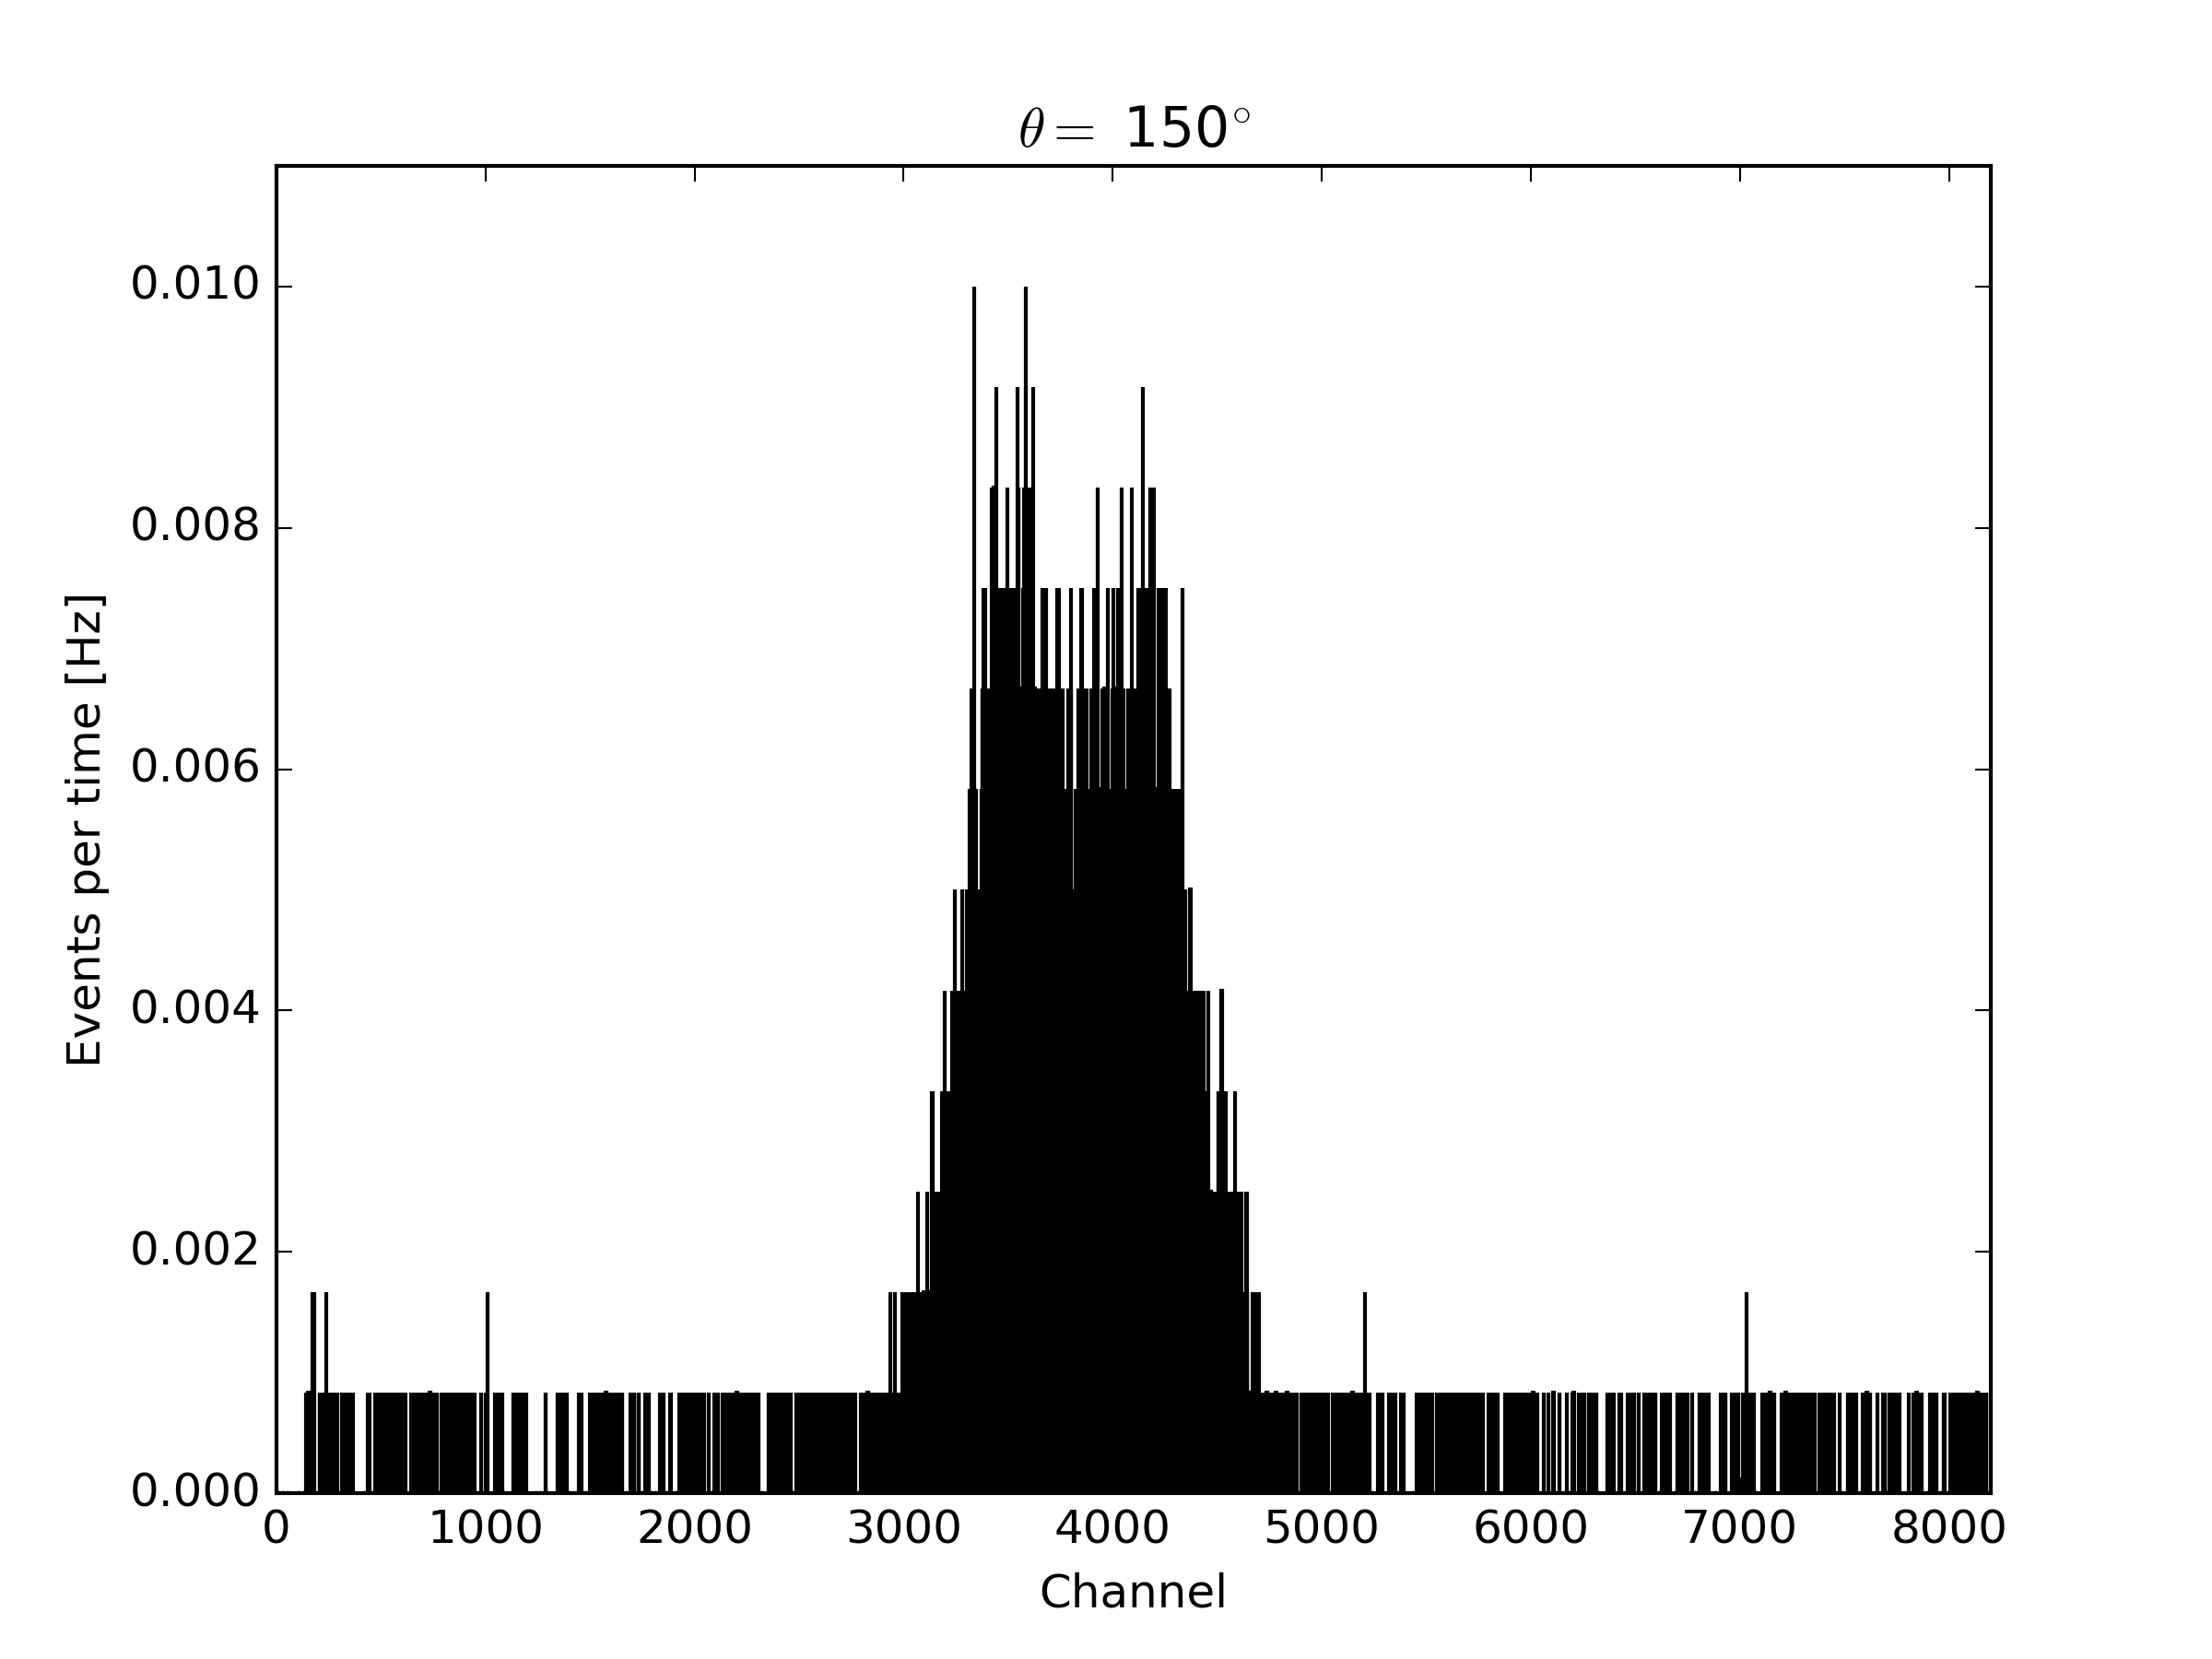
\includegraphics[width=0.33\textwidth]{150degraw.png}\hfill
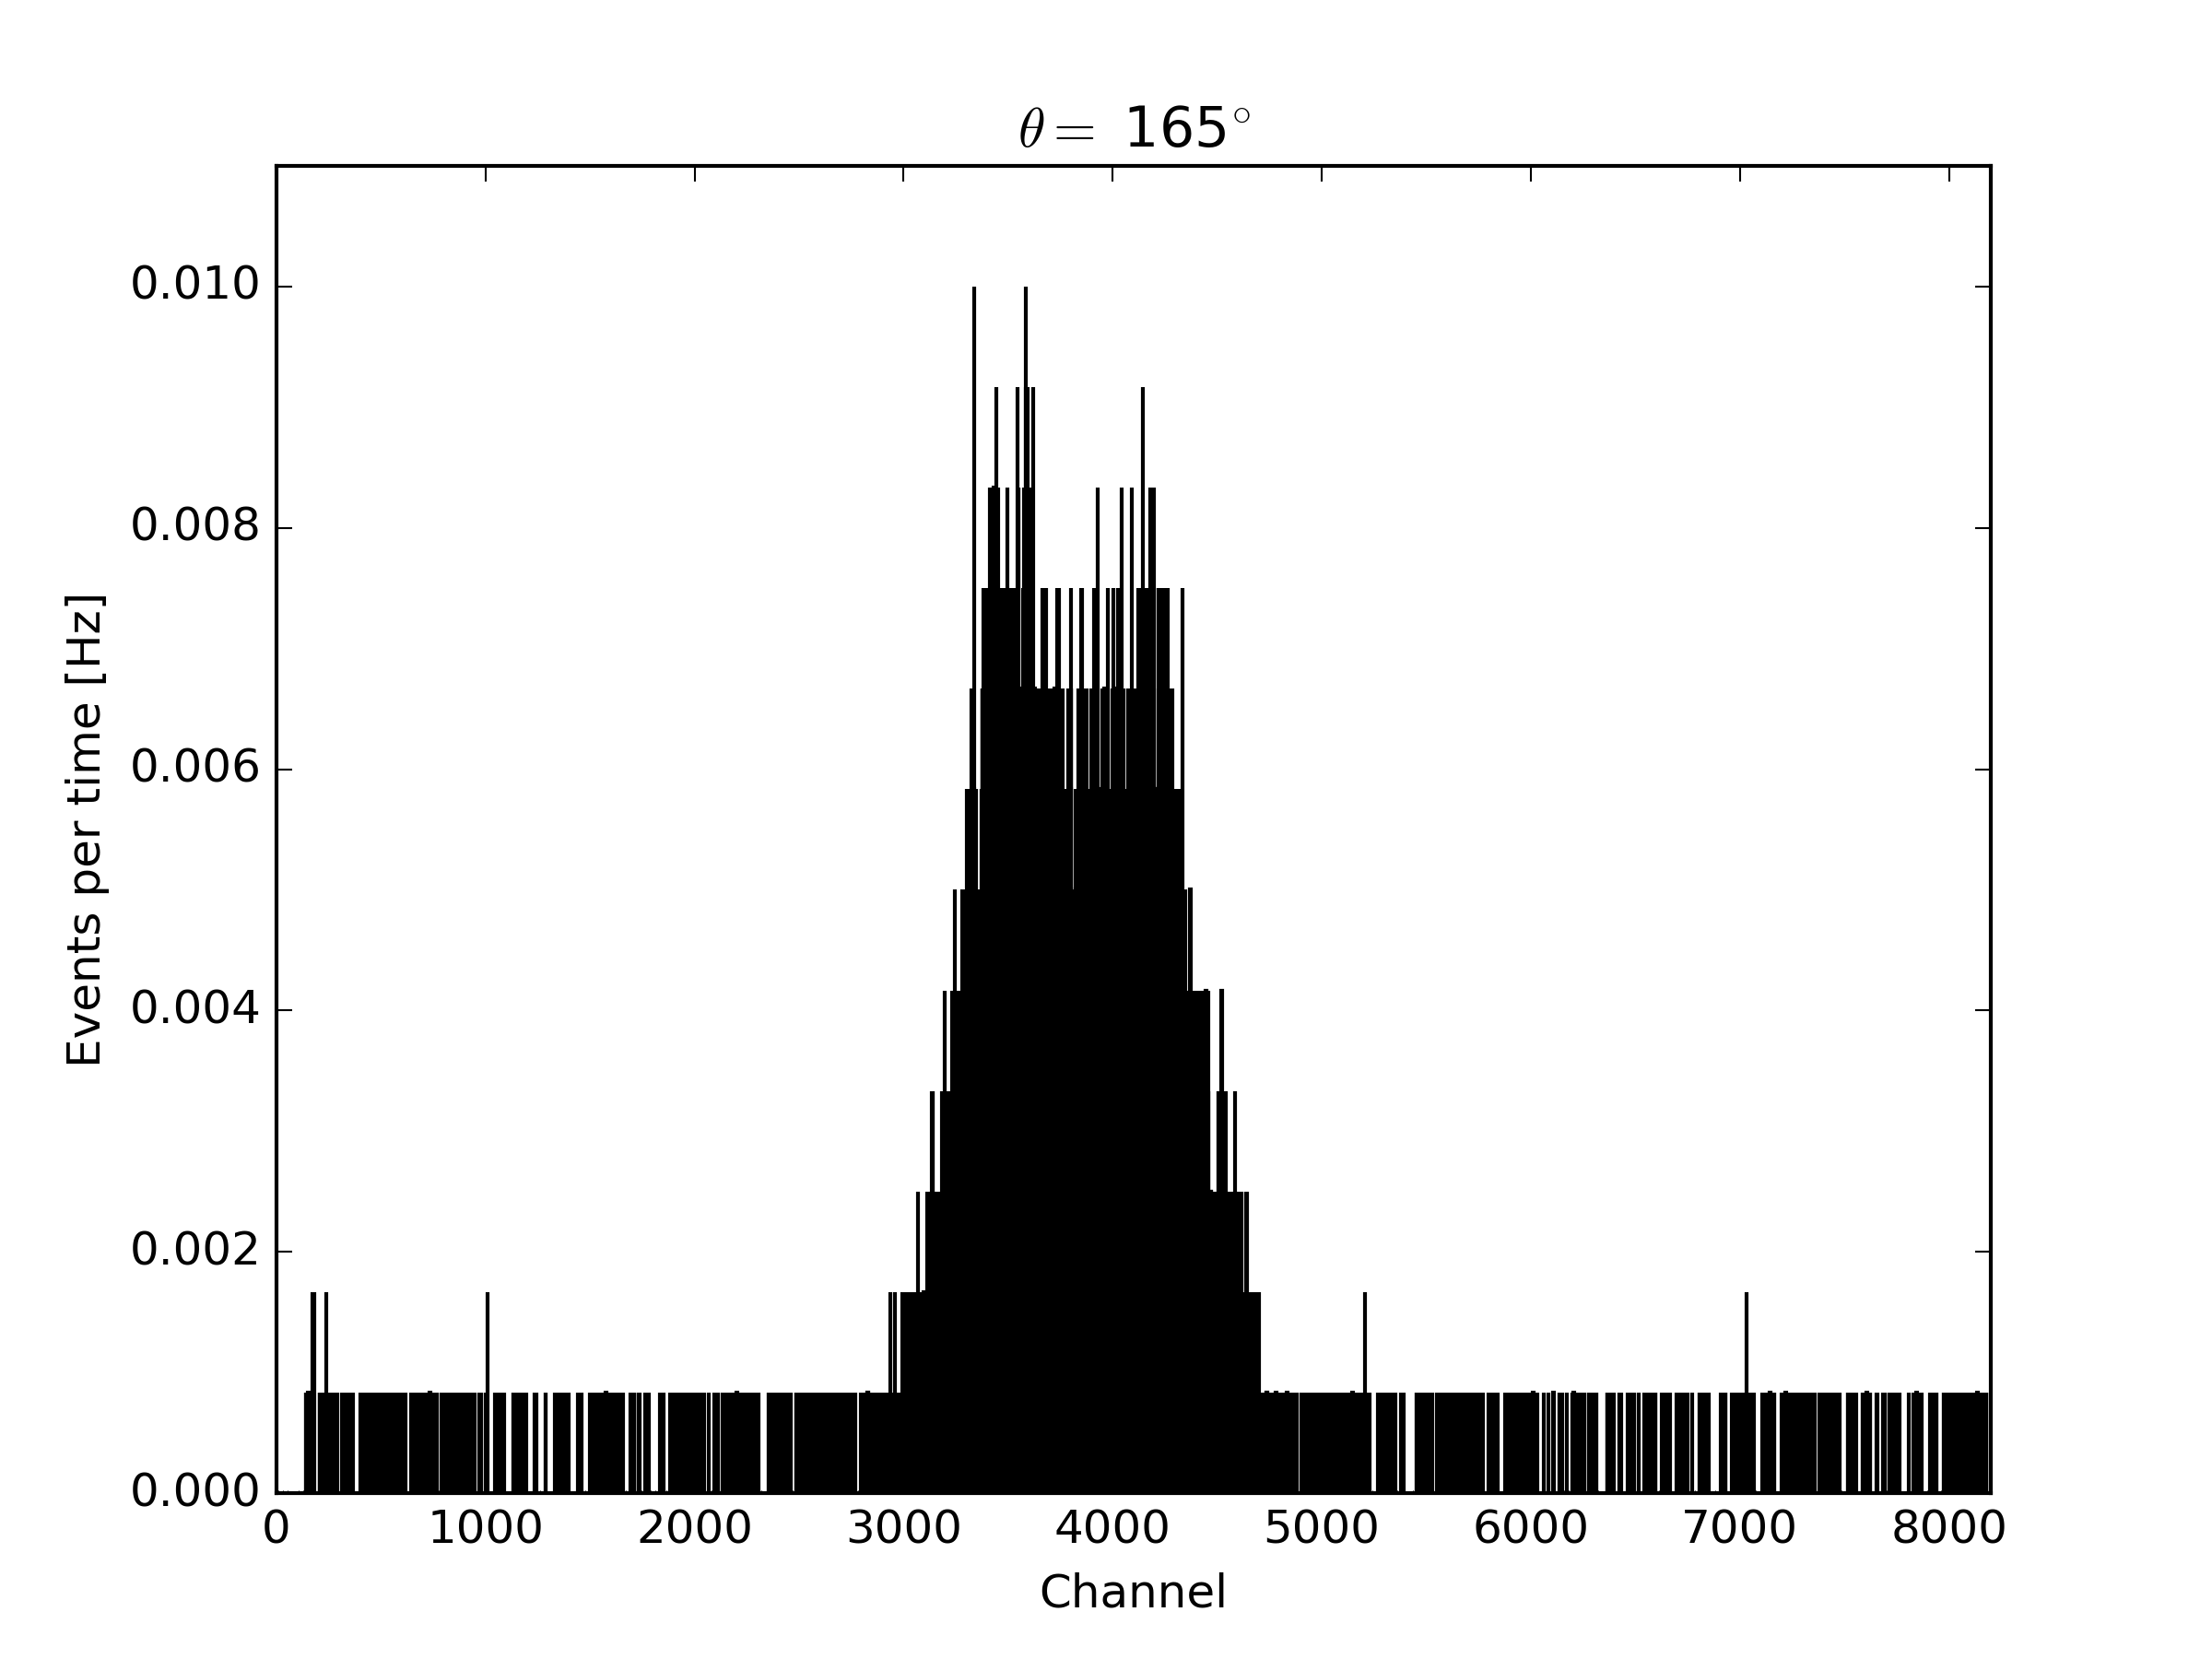
\includegraphics[width=0.33\textwidth]{165degraw.png}\hfill
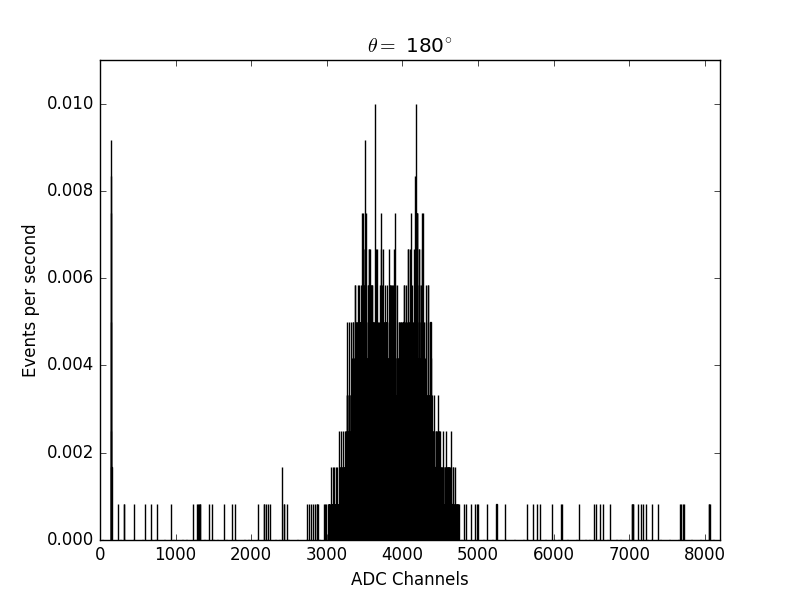
\includegraphics[width=0.33\textwidth]{180degraw.png}
\caption{Histograms with ADC channels for all angles}
\end{figure}
%

\section{Data Analysis}\label{app:histogram}
%
\begin{figure}[H]
\centering
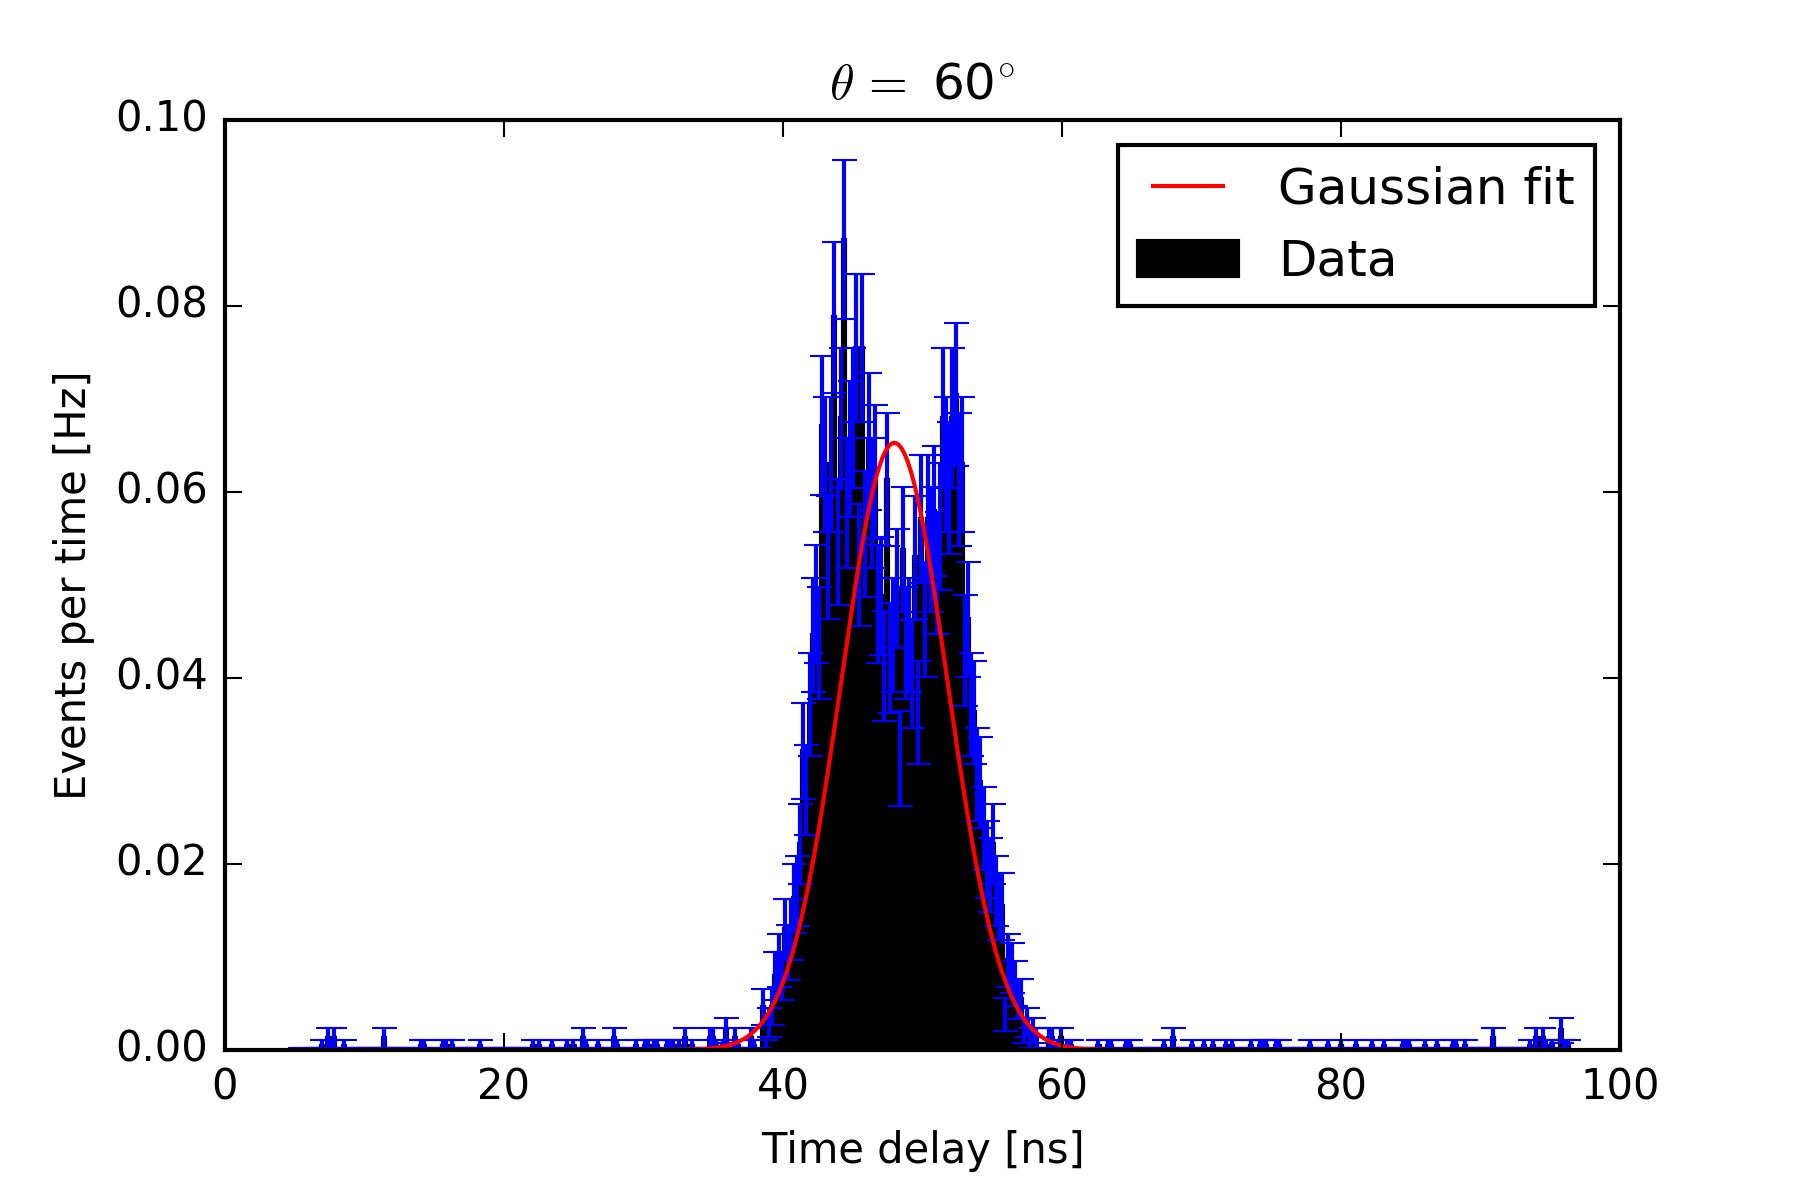
\includegraphics[width=0.33\textwidth]{60deg.png}\hfill
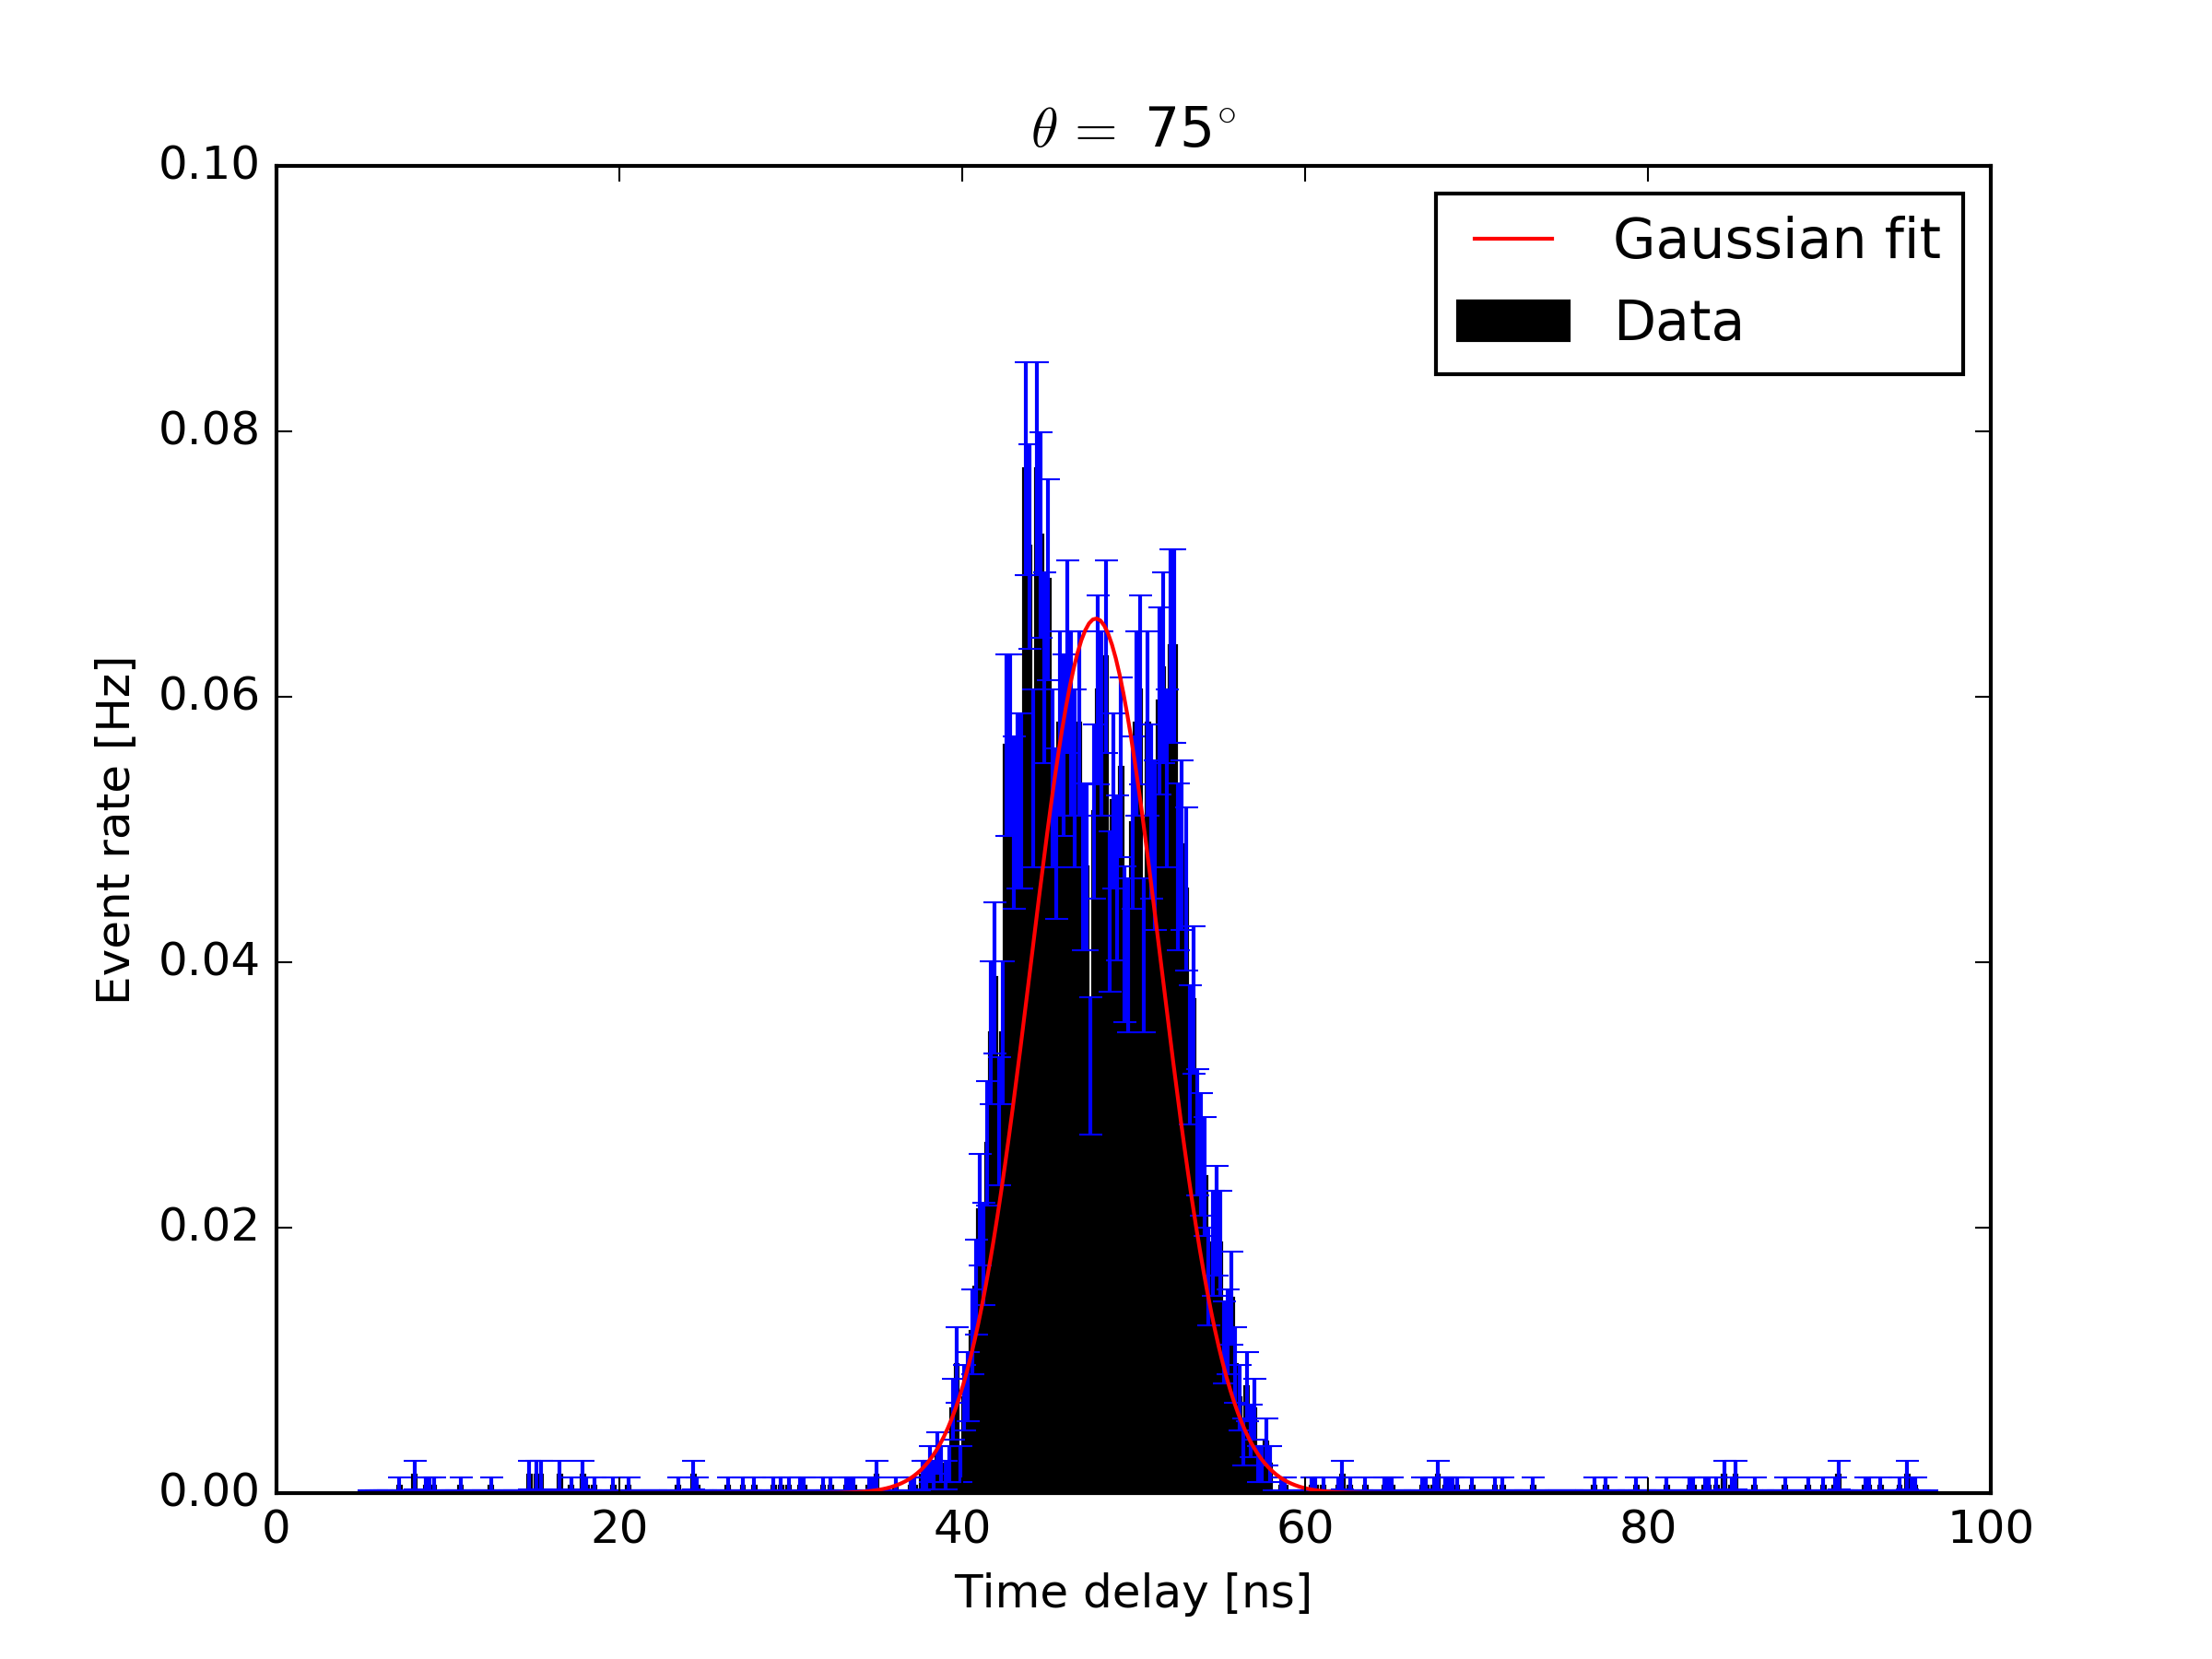
\includegraphics[width=0.33\textwidth]{75deg.png}\hfill
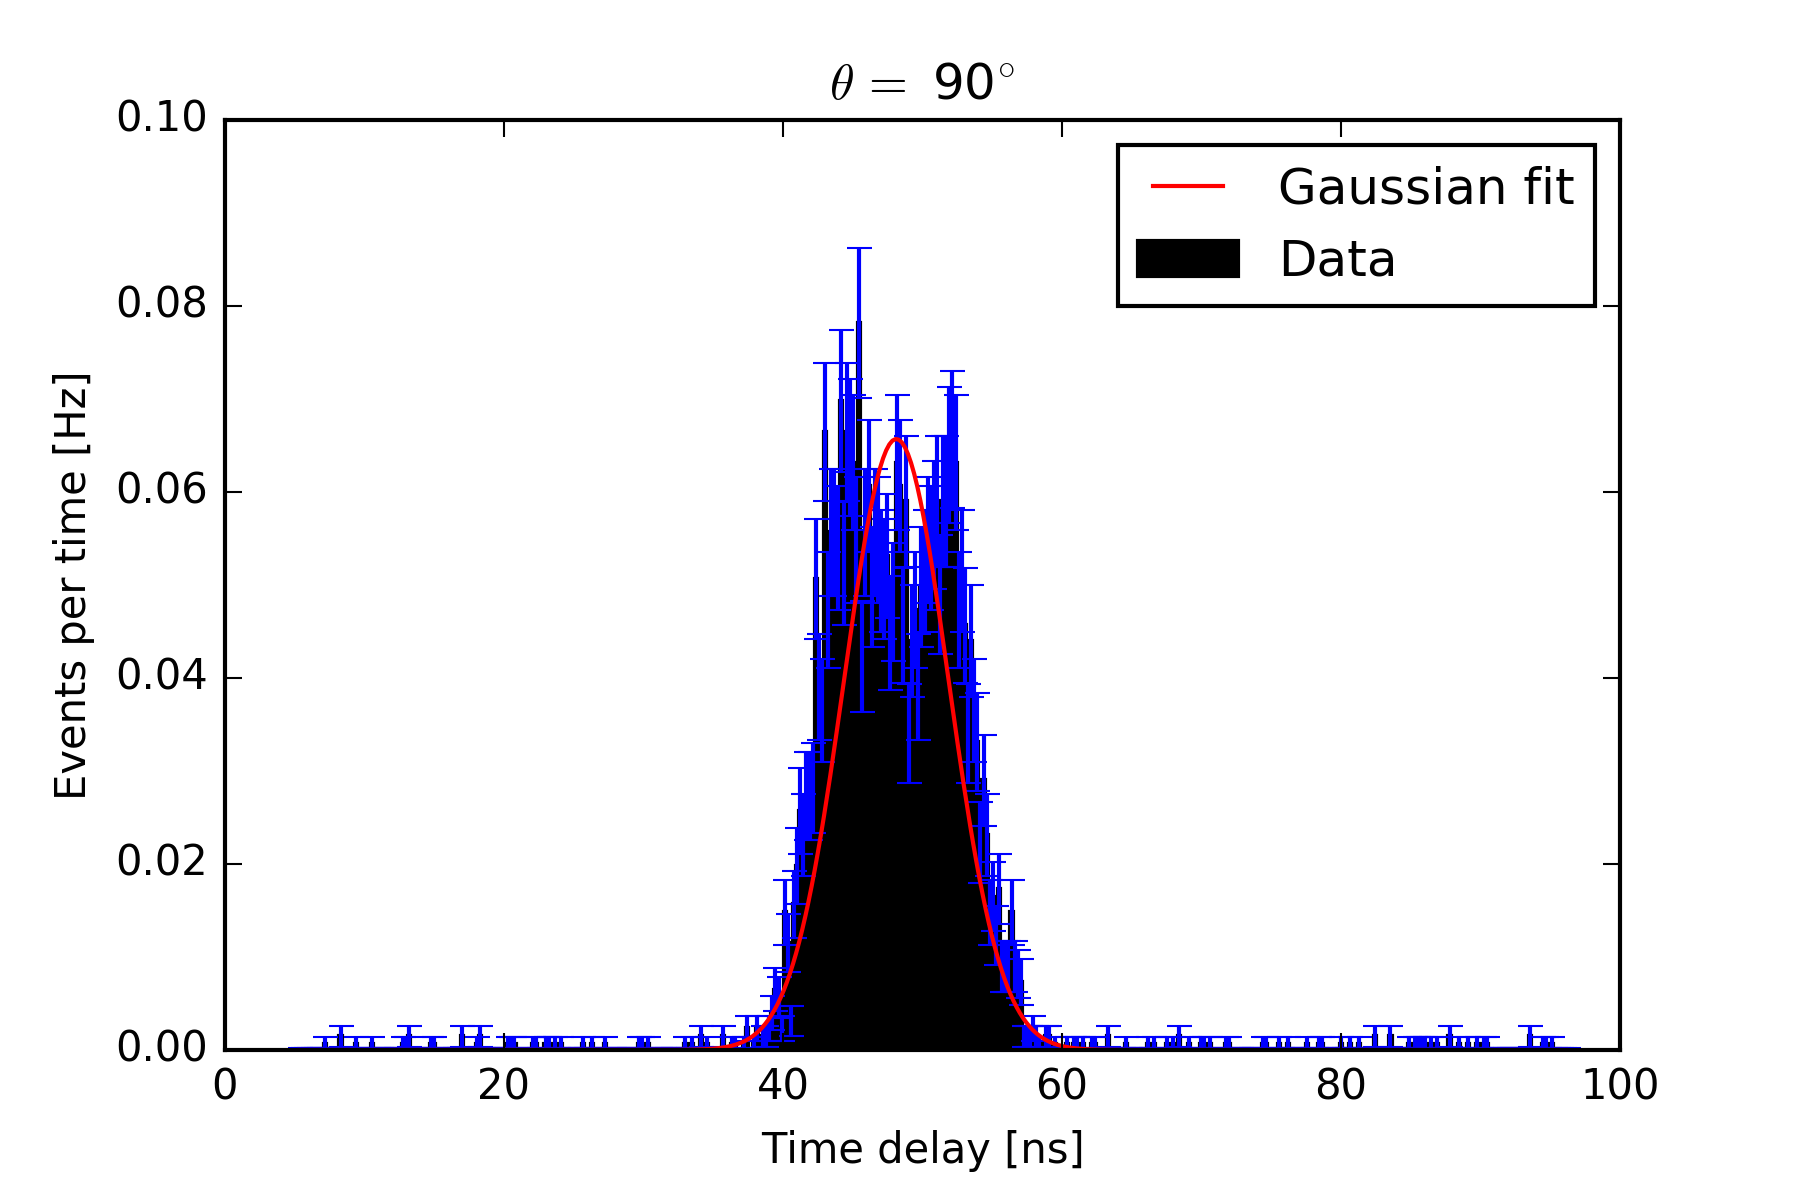
\includegraphics[width=0.33\textwidth]{90deg.png}\\
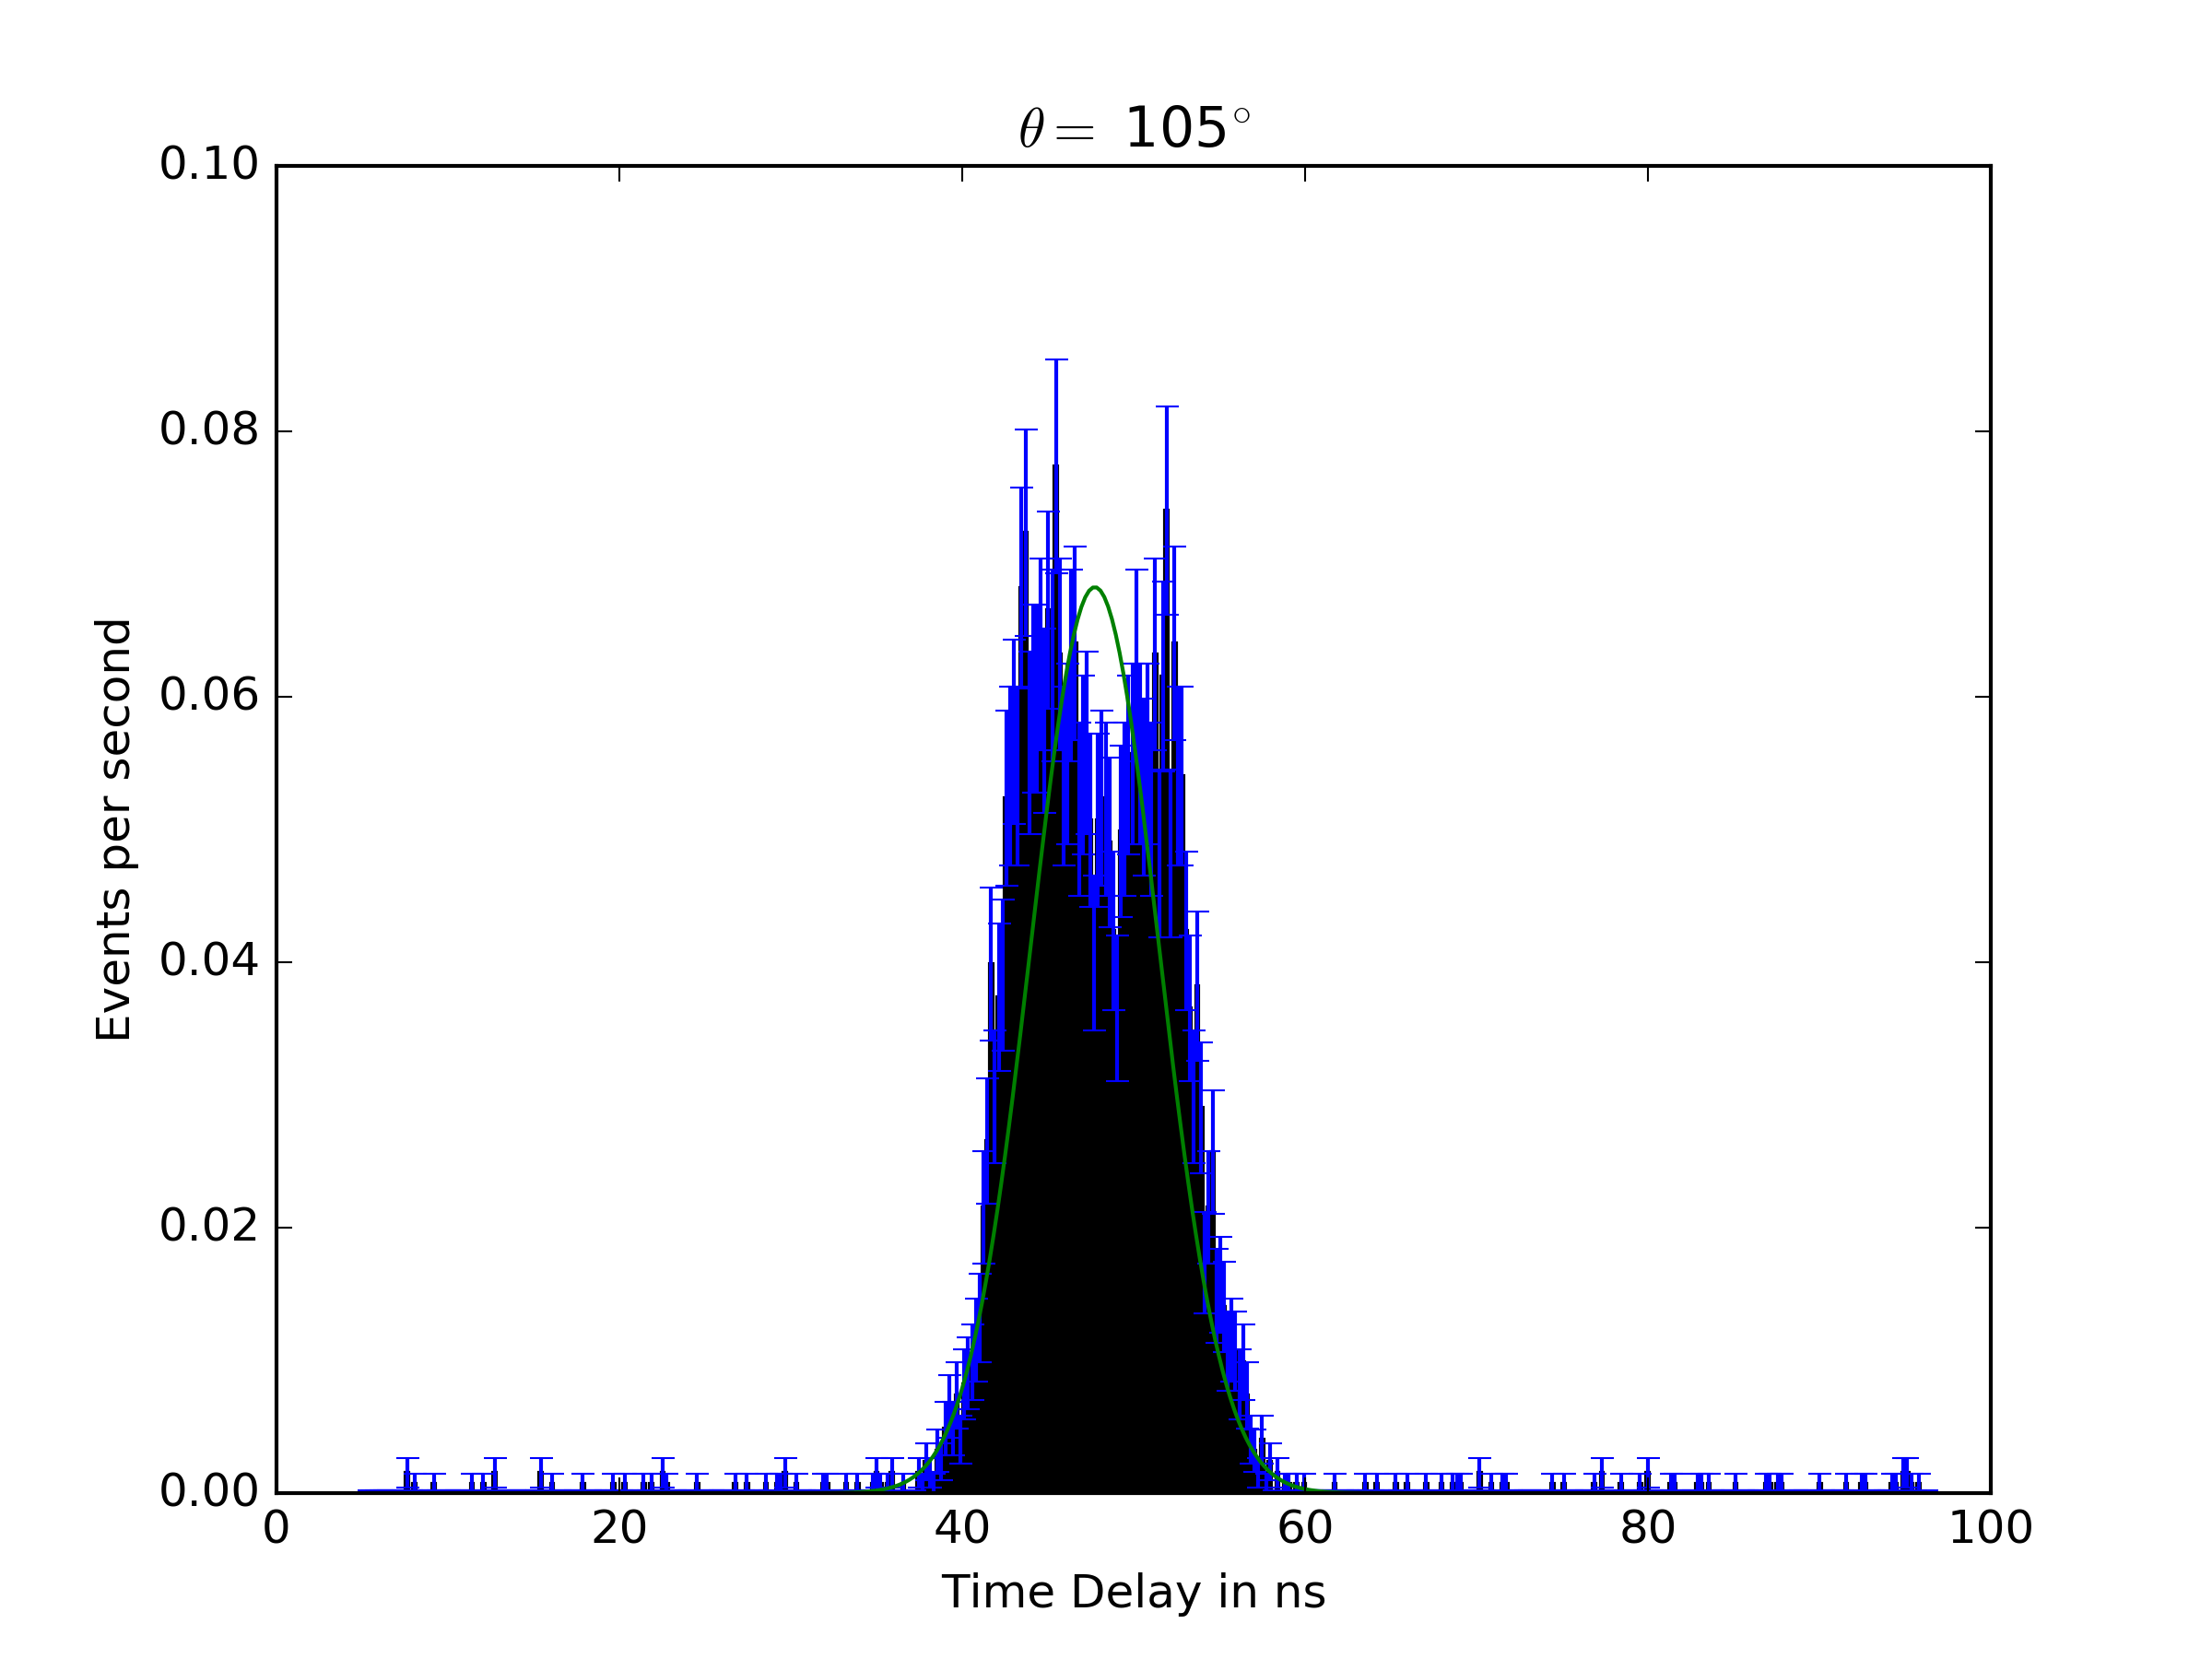
\includegraphics[width=0.33\textwidth]{105deg.png}\hfill
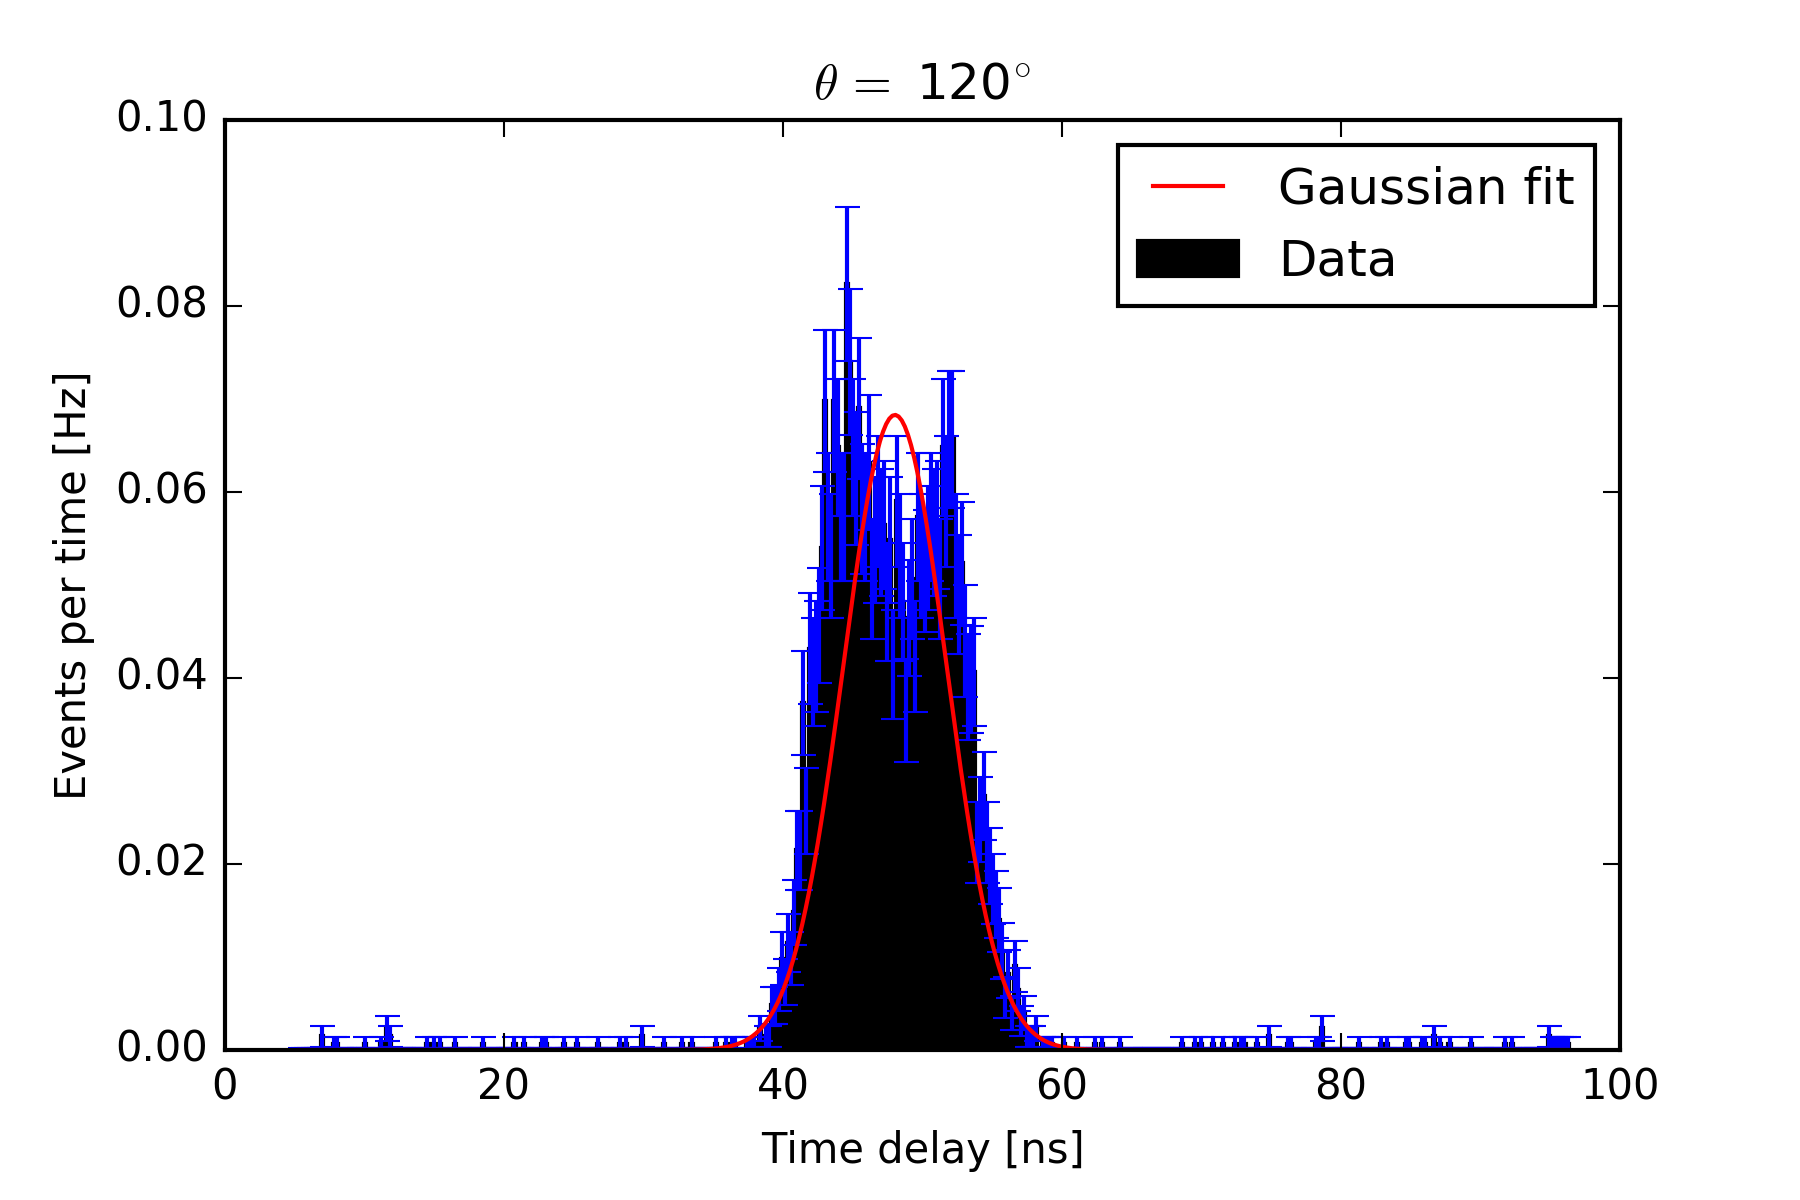
\includegraphics[width=0.33\textwidth]{120deg.png}\hfill
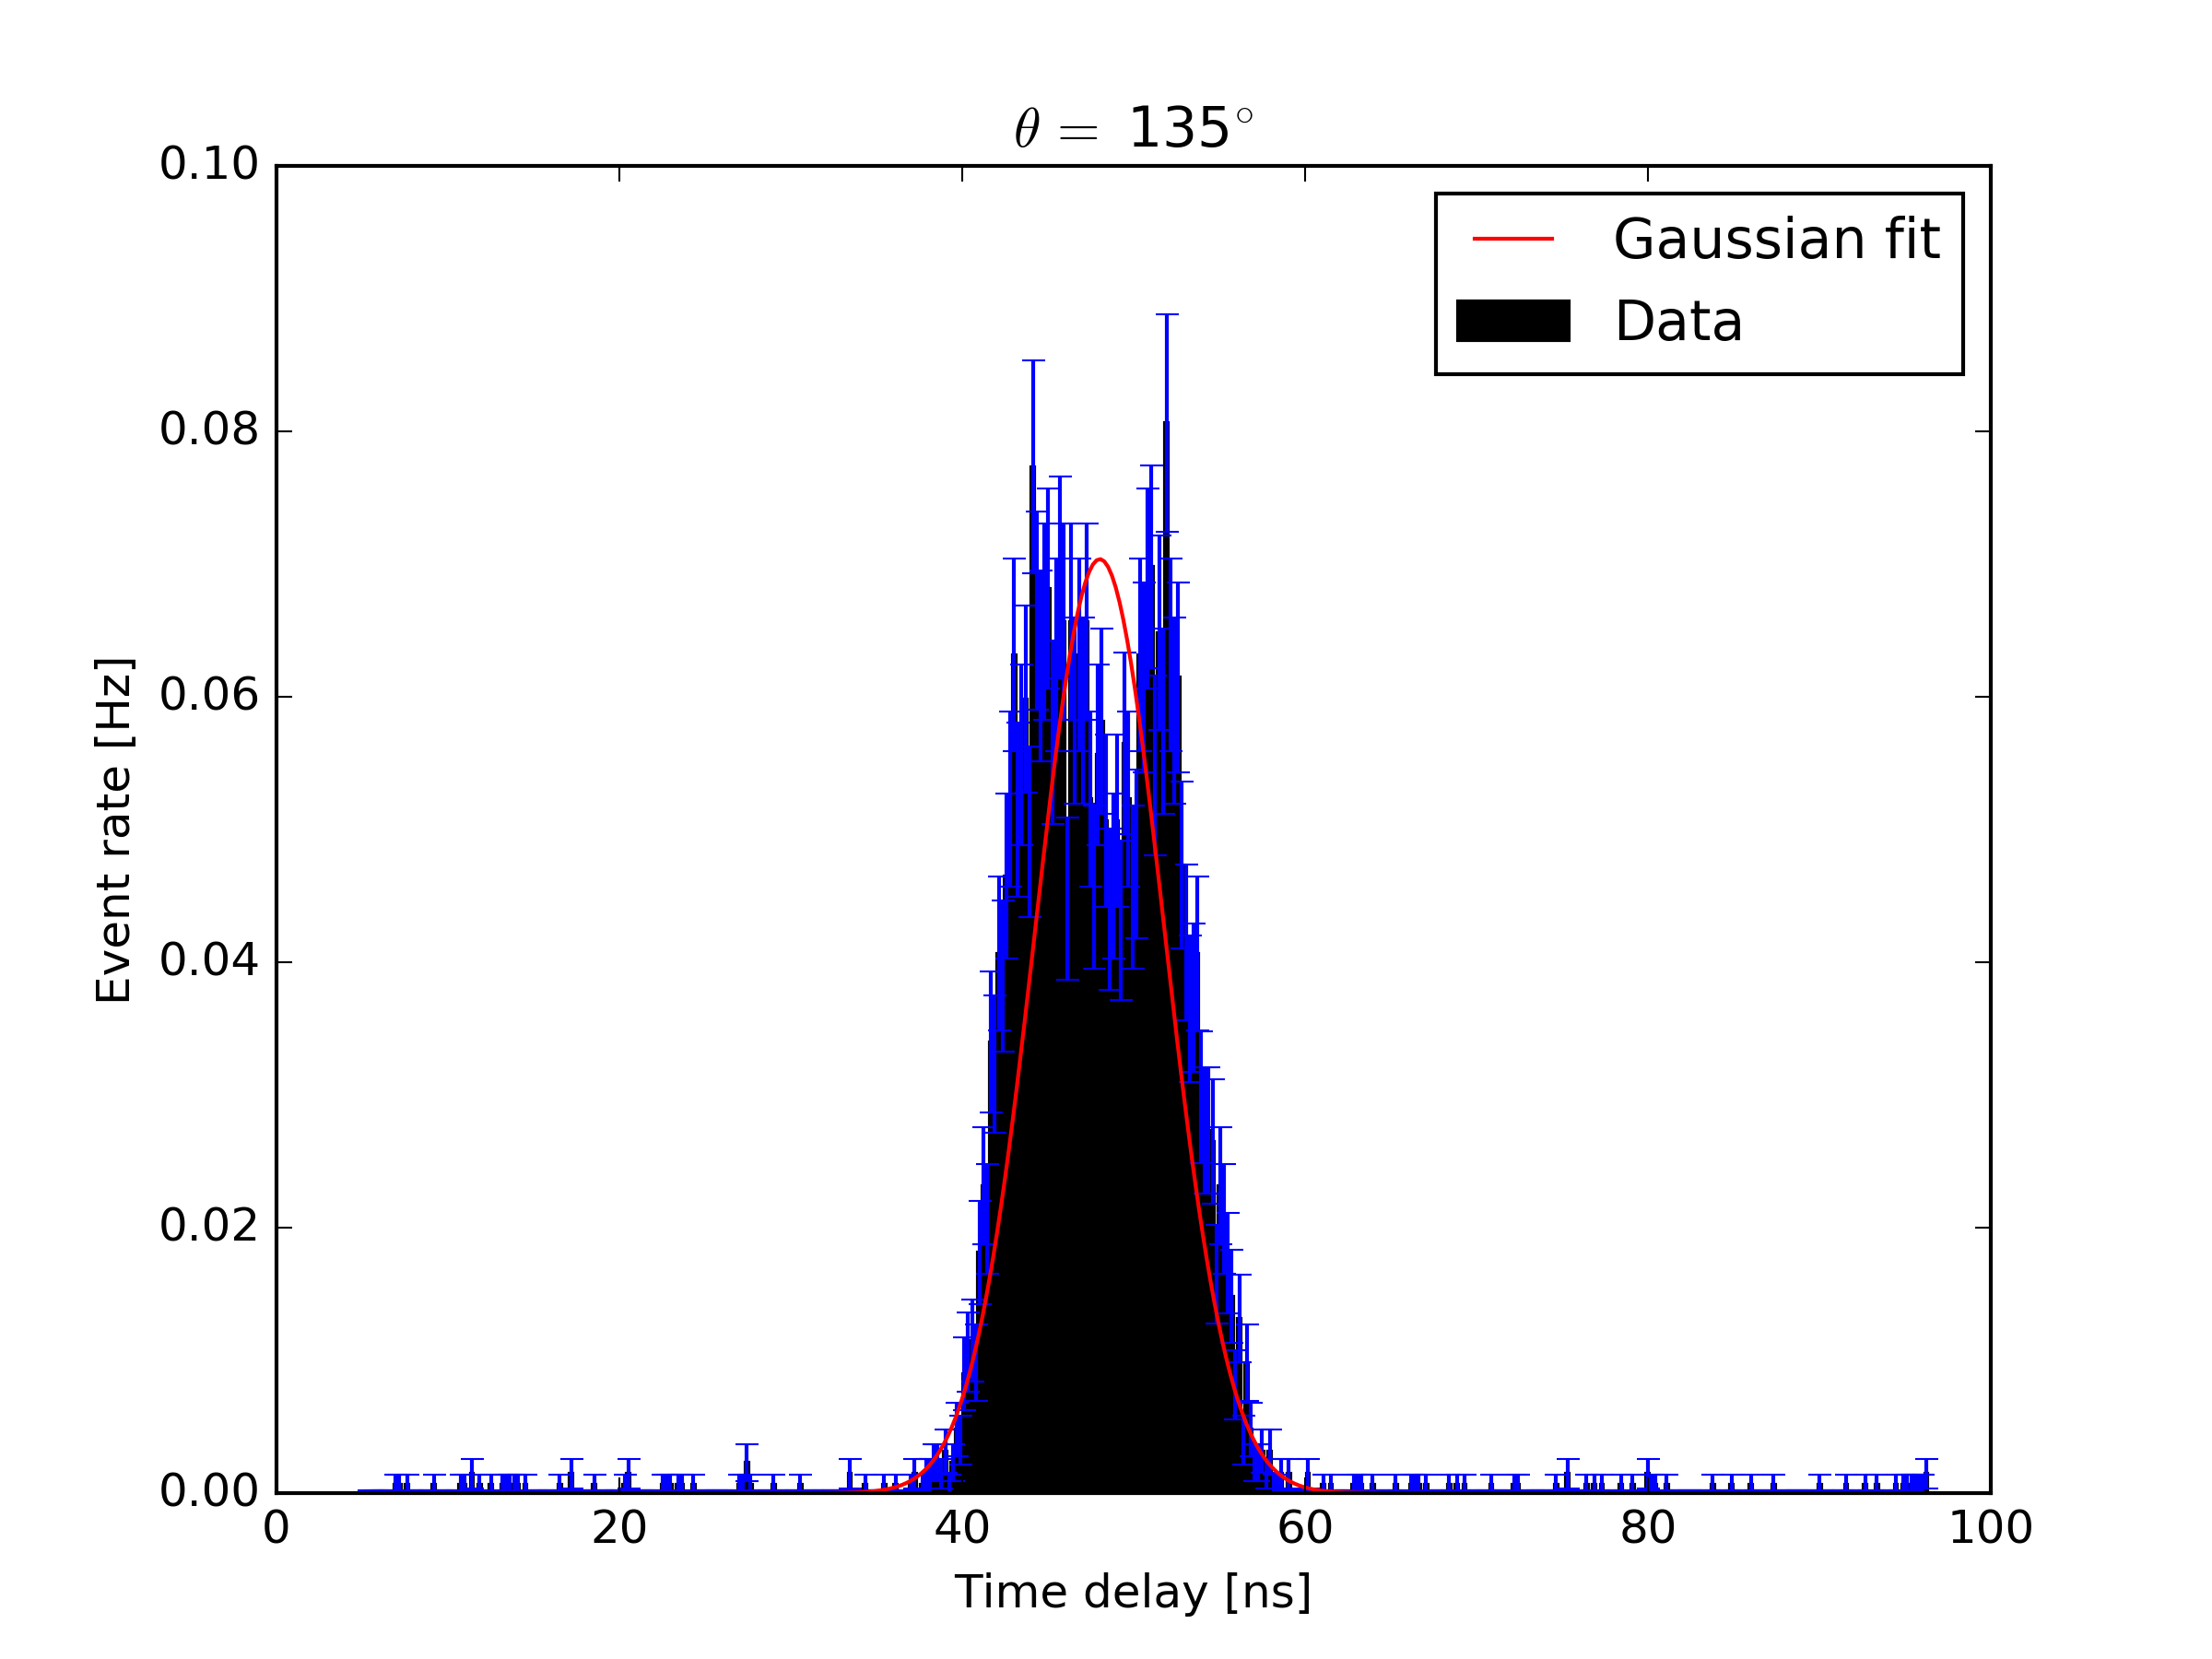
\includegraphics[width=0.33\textwidth]{135deg.png}\\
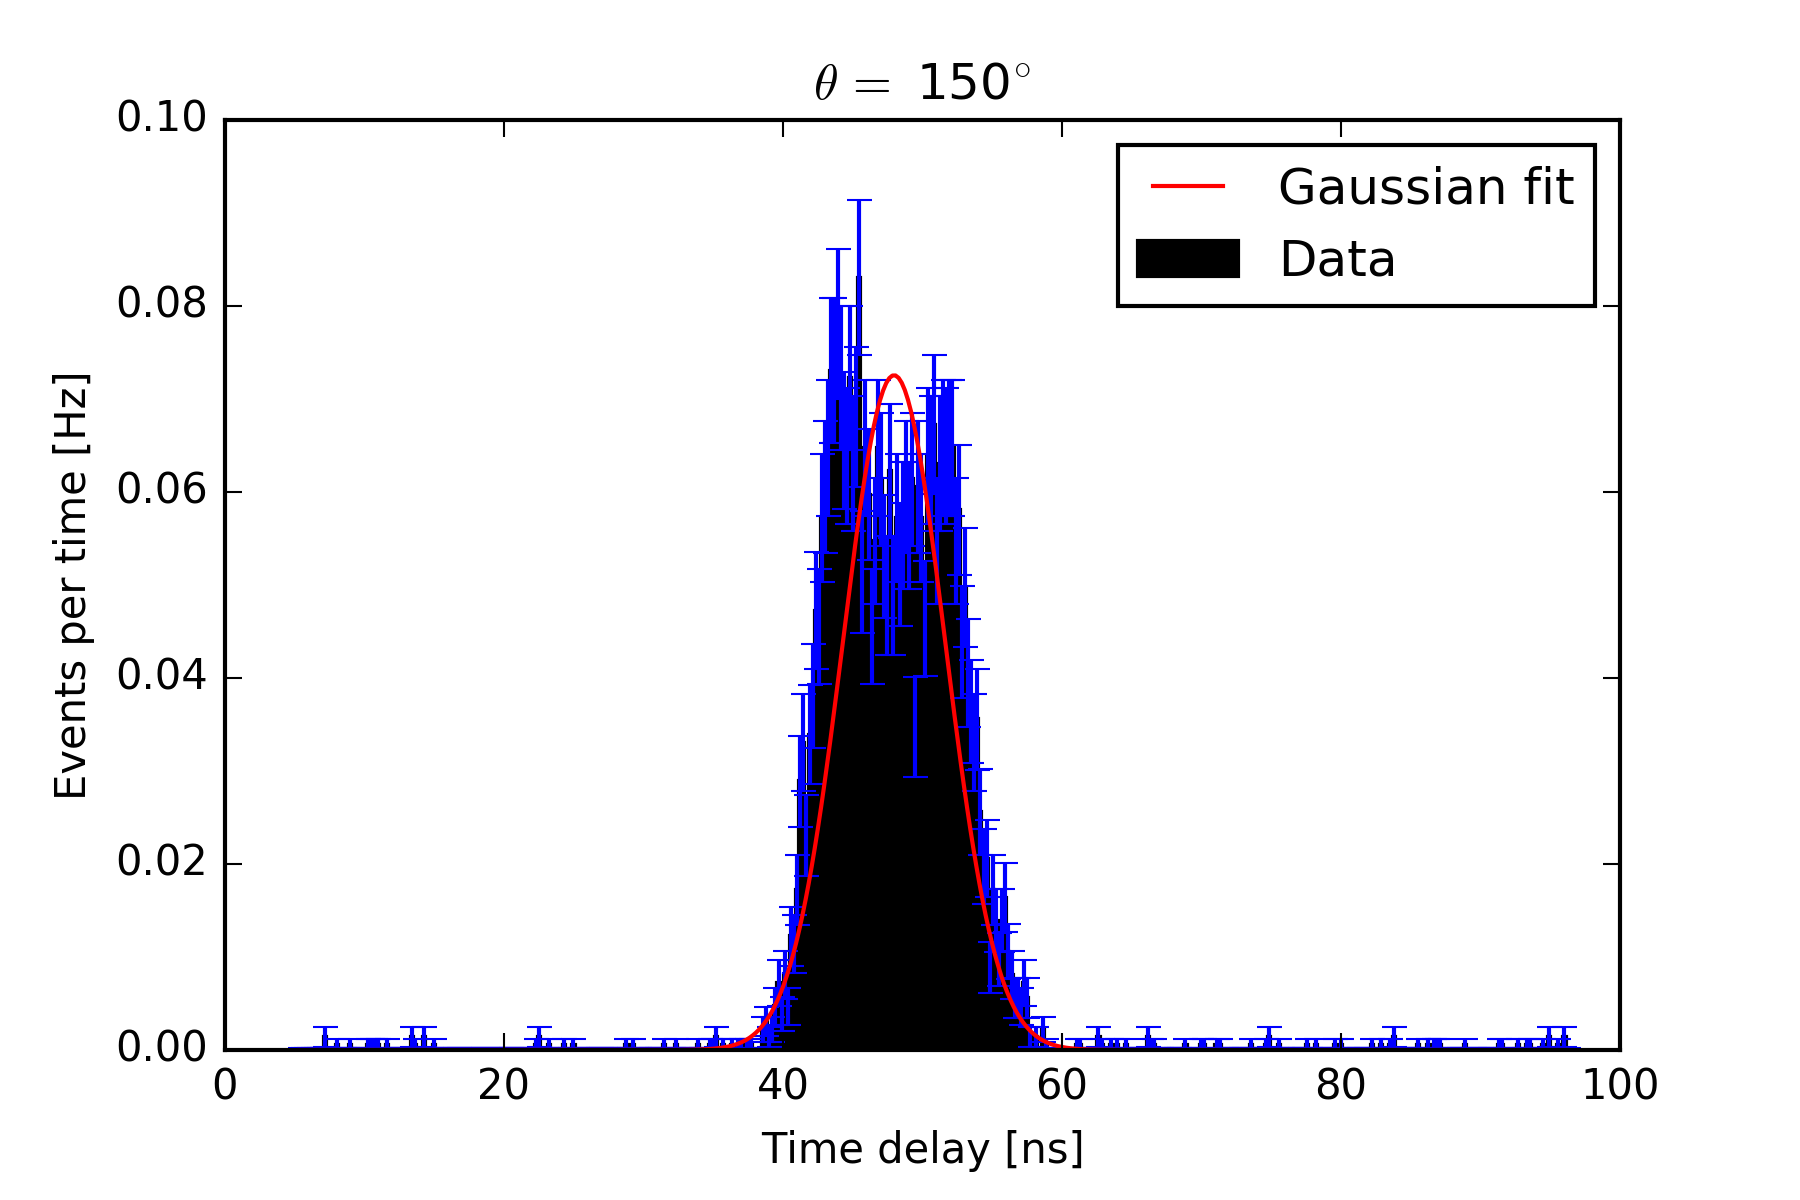
\includegraphics[width=0.33\textwidth]{150deg.png}\hfill
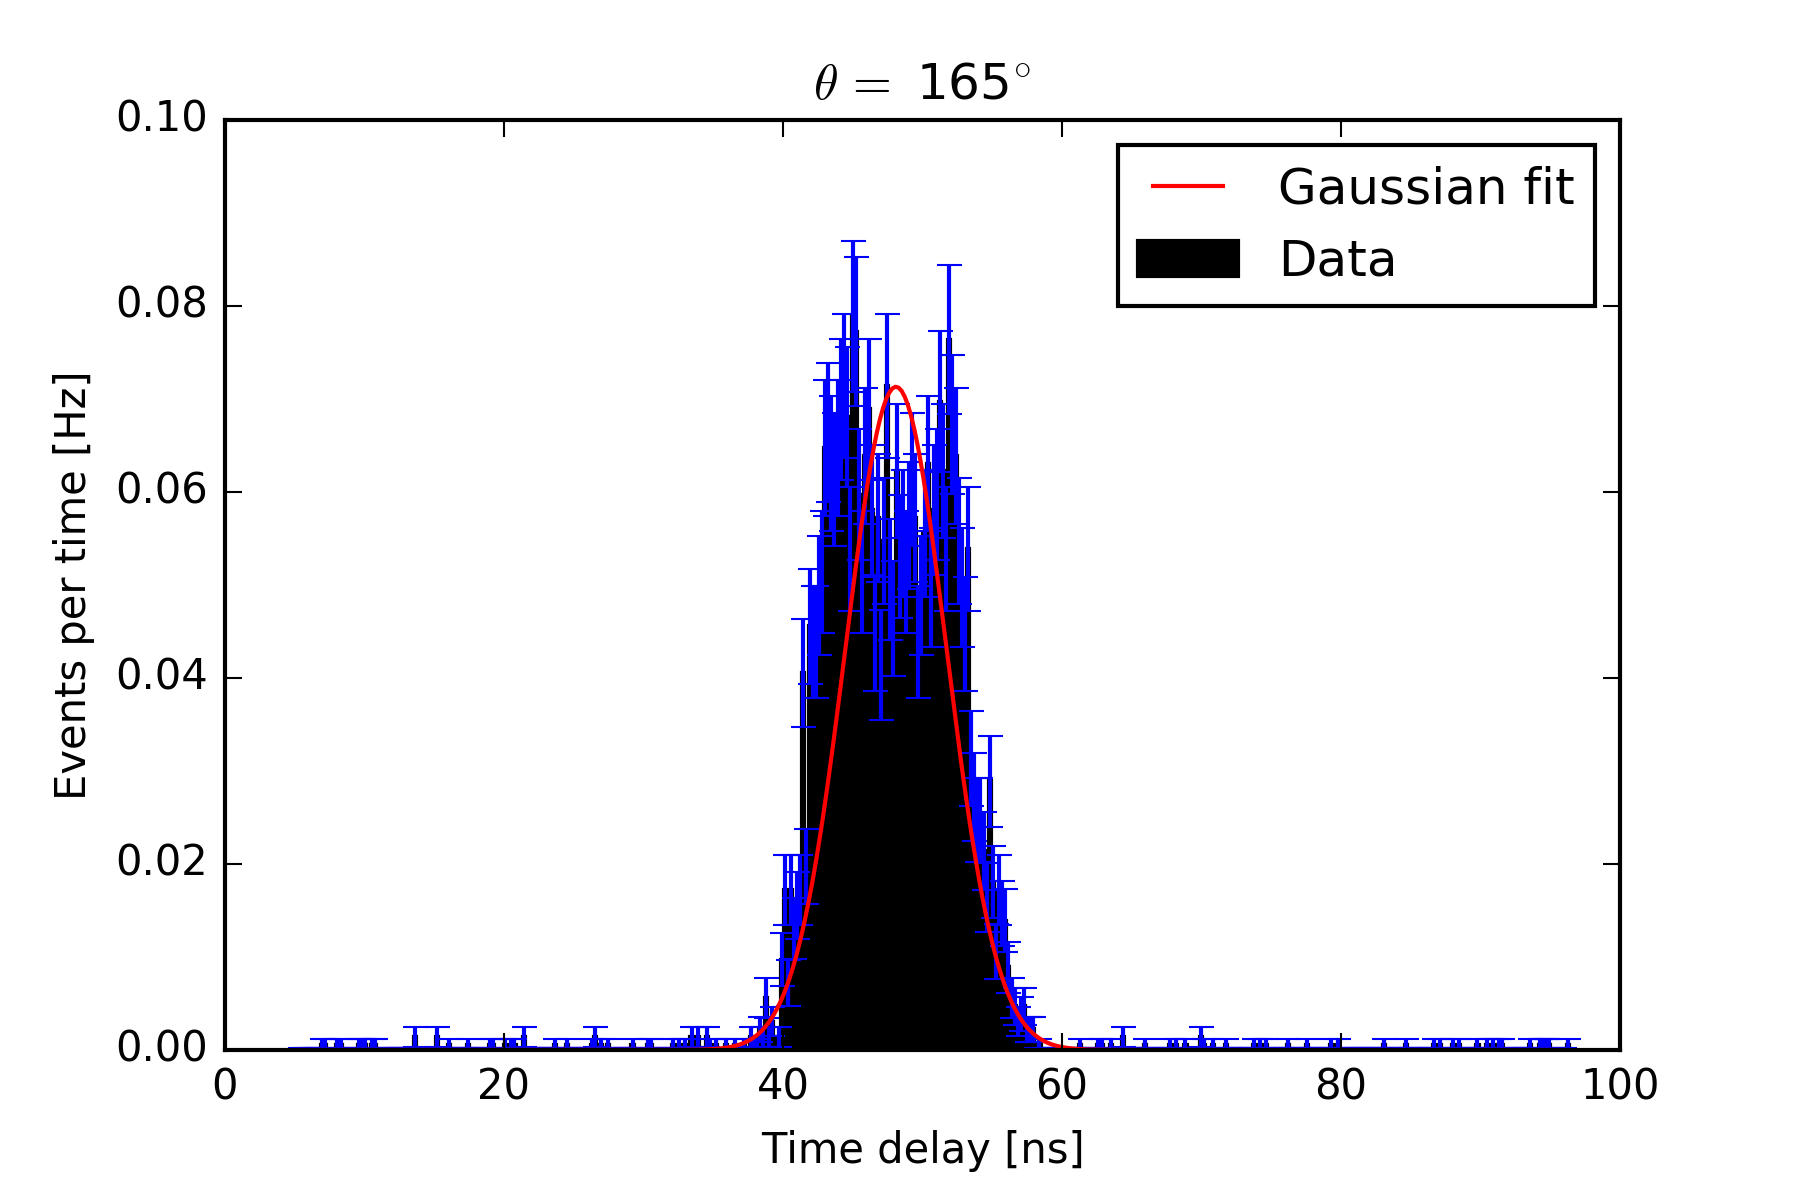
\includegraphics[width=0.33\textwidth]{165deg.png}\hfill
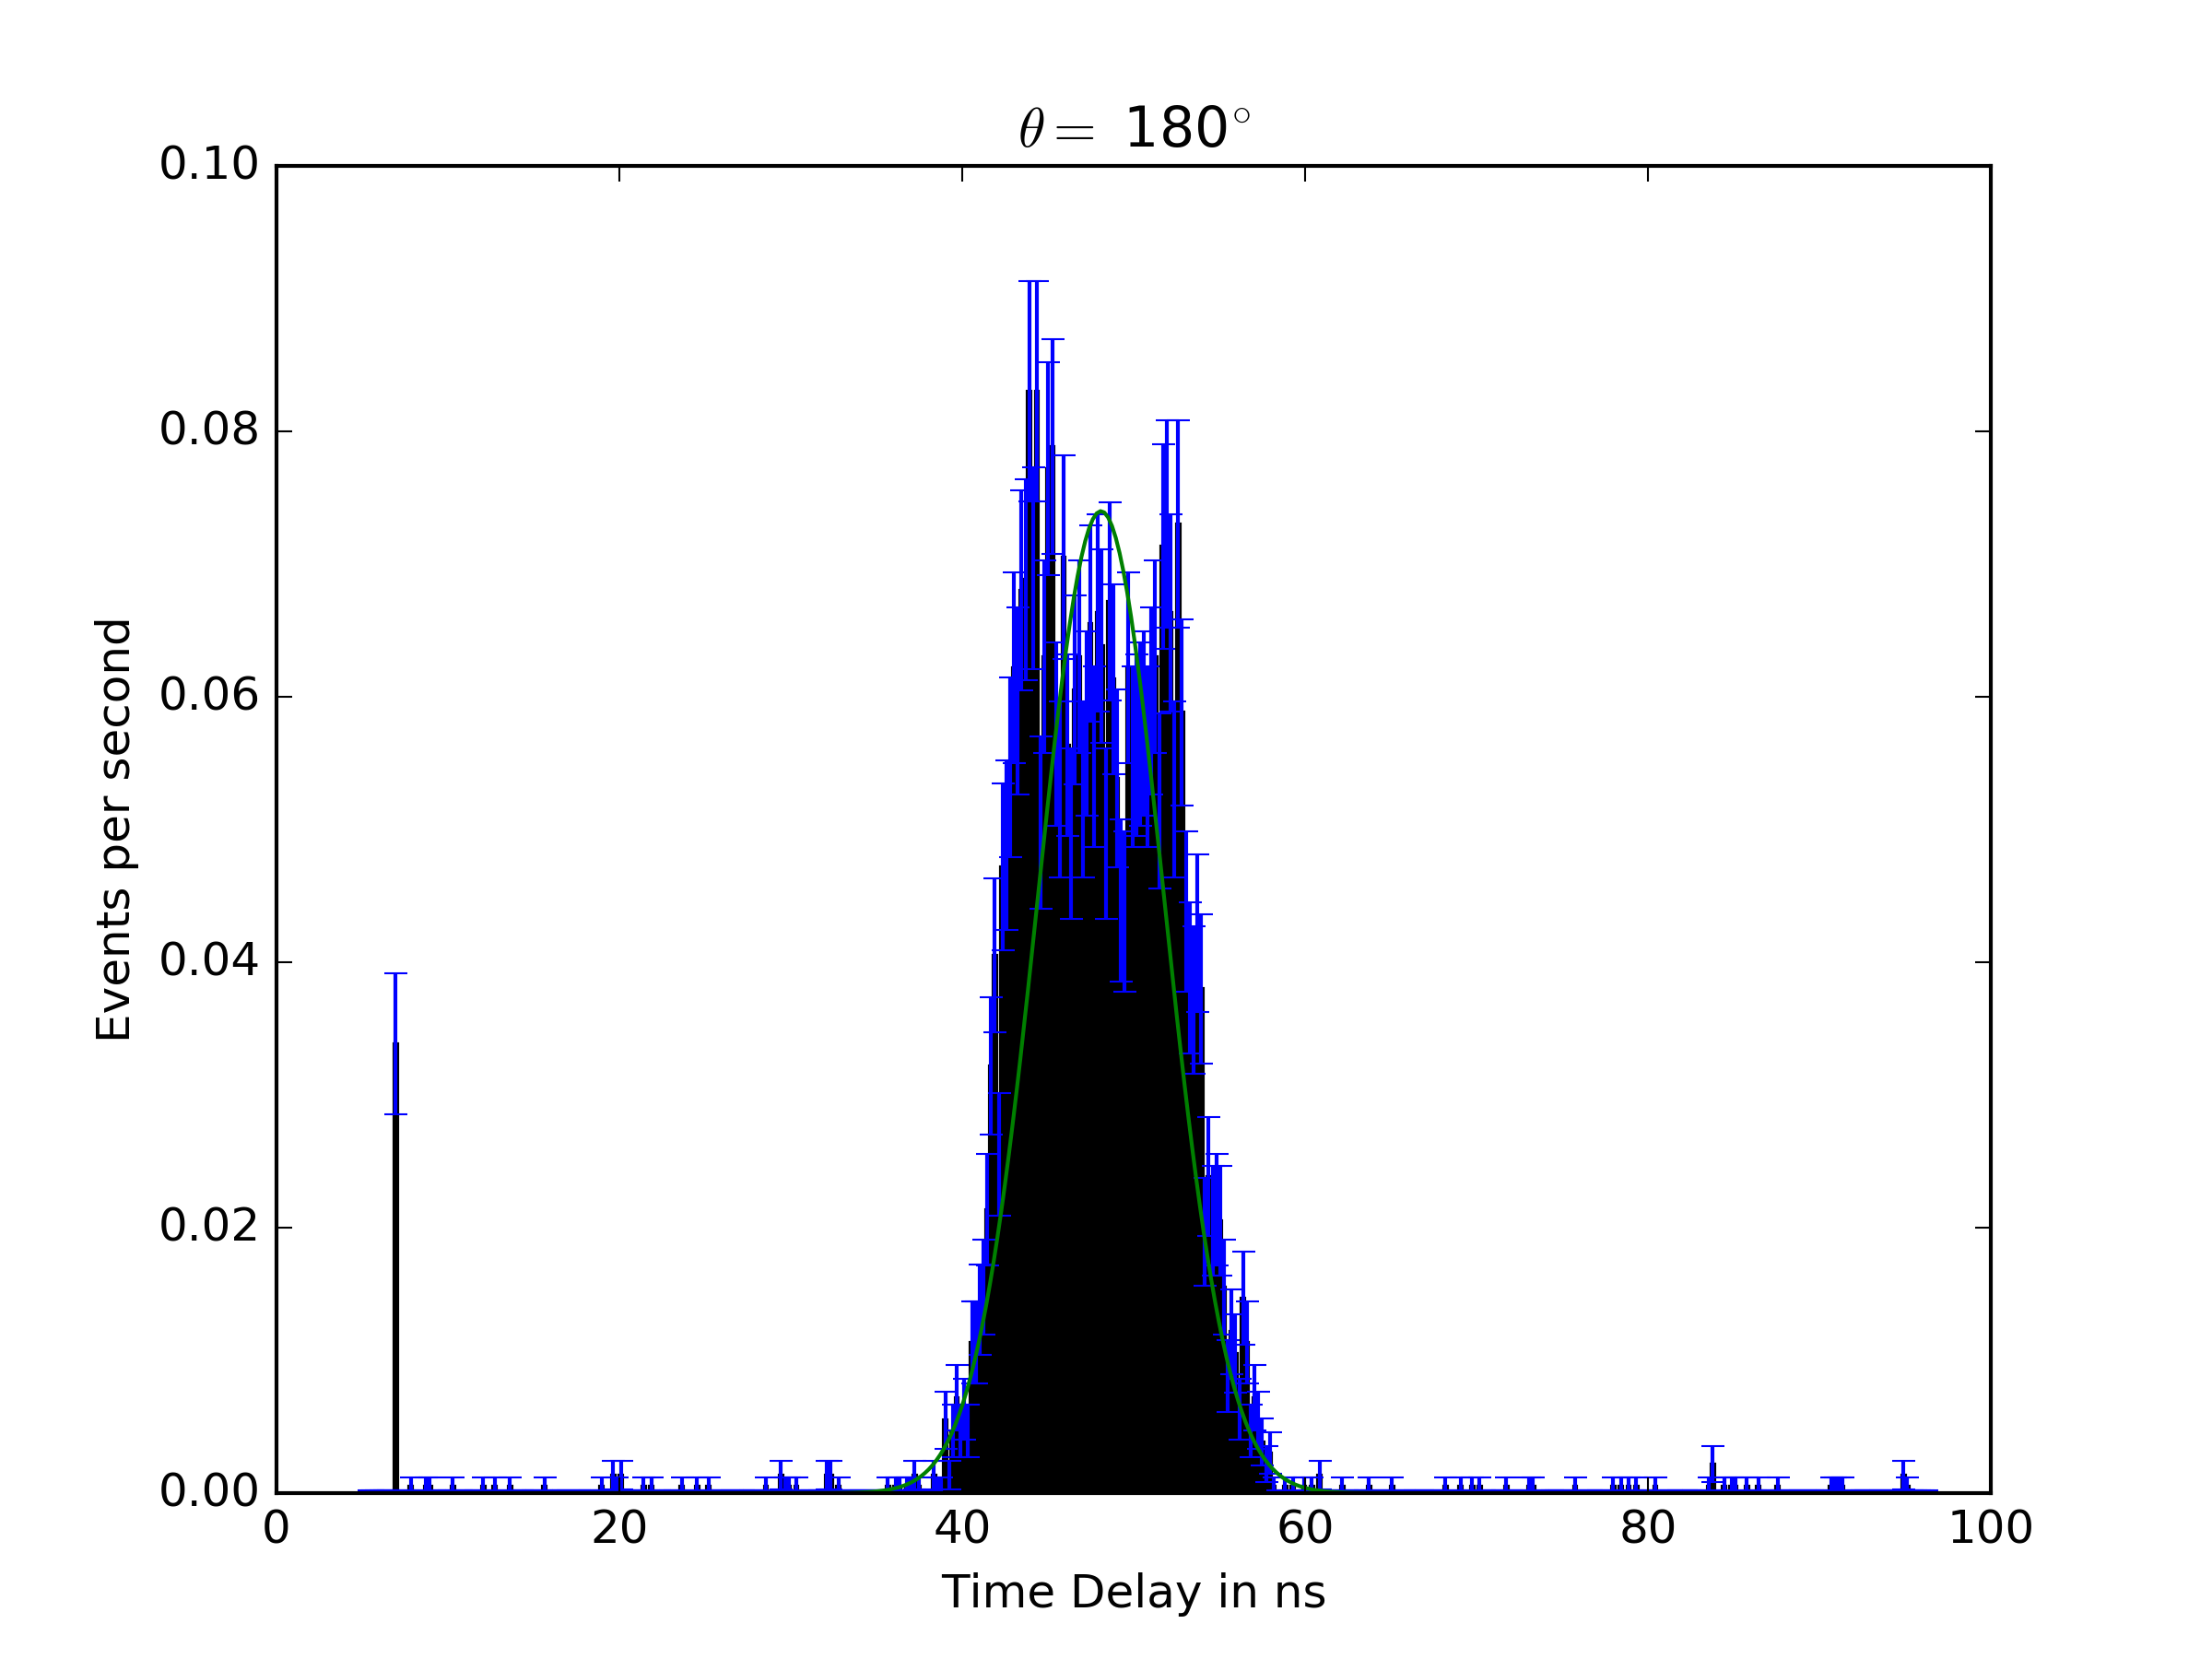
\includegraphics[width=0.33\textwidth]{180deg.png}
\caption{Rebinned histograms on time axis with background subtracted and fitted Gaussian for all angles}
\end{figure}


\section{References}

[\ref{source:manual}]: Instruction manual and assistants \labeltext{1}{source:manual}

[\ref{source:Hamilton}]: Donald R. Hamilton Phys. Rev. 58, 122 (1940) \labeltext{2}{source:Hamilton}

[\ref{source:WilliamLeo}]: Dr. William R. Leo - Techniques for Nuclear and Particle Physics Experiments: A How-to Approach (1994)\labeltext{3}{source:WilliamLeo}

[\ref{source:GlennKnoll}]: Glenn F. Knoll - Radiation Detection and Measurement (2010) \labeltext{4}{source:GlennKnoll}



%Donald R. Hamilton Phys. Rev. 58, 122 (1940)



%Compton Edge Formula, Source: Glenn F. Knoll-Radiation Detection and Measurement-Wiley (2010)

%Dr. William R. Leo (auth.)-Techniques for Nuclear and Particle Physics Experiments_ A How-to Approach-Springer-Verlag Berlin Heidelberg (1994)

%https://journals.aps.org/pr/pdf/10.1103/PhysRev.78.558

%https://journals.aps.org/pr/pdf/10.1103/PhysRev.58.122

%Instruction manual and assistant


\end{document}
